% Options for packages loaded elsewhere
% Options for packages loaded elsewhere
\PassOptionsToPackage{unicode}{hyperref}
\PassOptionsToPackage{hyphens}{url}
\PassOptionsToPackage{dvipsnames,svgnames,x11names}{xcolor}
%
\documentclass[
  letterpaper,
  DIV=11,
  numbers=noendperiod]{scrartcl}
\usepackage{xcolor}
\usepackage[top=30mm,left=30mm]{geometry}
\usepackage{amsmath,amssymb}
\setcounter{secnumdepth}{-\maxdimen} % remove section numbering
\usepackage{iftex}
\ifPDFTeX
  \usepackage[T1]{fontenc}
  \usepackage[utf8]{inputenc}
  \usepackage{textcomp} % provide euro and other symbols
\else % if luatex or xetex
  \usepackage{unicode-math} % this also loads fontspec
  \defaultfontfeatures{Scale=MatchLowercase}
  \defaultfontfeatures[\rmfamily]{Ligatures=TeX,Scale=1}
\fi
\usepackage{lmodern}
\ifPDFTeX\else
  % xetex/luatex font selection
\fi
% Use upquote if available, for straight quotes in verbatim environments
\IfFileExists{upquote.sty}{\usepackage{upquote}}{}
\IfFileExists{microtype.sty}{% use microtype if available
  \usepackage[]{microtype}
  \UseMicrotypeSet[protrusion]{basicmath} % disable protrusion for tt fonts
}{}
\makeatletter
\@ifundefined{KOMAClassName}{% if non-KOMA class
  \IfFileExists{parskip.sty}{%
    \usepackage{parskip}
  }{% else
    \setlength{\parindent}{0pt}
    \setlength{\parskip}{6pt plus 2pt minus 1pt}}
}{% if KOMA class
  \KOMAoptions{parskip=half}}
\makeatother
% Make \paragraph and \subparagraph free-standing
\makeatletter
\ifx\paragraph\undefined\else
  \let\oldparagraph\paragraph
  \renewcommand{\paragraph}{
    \@ifstar
      \xxxParagraphStar
      \xxxParagraphNoStar
  }
  \newcommand{\xxxParagraphStar}[1]{\oldparagraph*{#1}\mbox{}}
  \newcommand{\xxxParagraphNoStar}[1]{\oldparagraph{#1}\mbox{}}
\fi
\ifx\subparagraph\undefined\else
  \let\oldsubparagraph\subparagraph
  \renewcommand{\subparagraph}{
    \@ifstar
      \xxxSubParagraphStar
      \xxxSubParagraphNoStar
  }
  \newcommand{\xxxSubParagraphStar}[1]{\oldsubparagraph*{#1}\mbox{}}
  \newcommand{\xxxSubParagraphNoStar}[1]{\oldsubparagraph{#1}\mbox{}}
\fi
\makeatother

\usepackage{color}
\usepackage{fancyvrb}
\newcommand{\VerbBar}{|}
\newcommand{\VERB}{\Verb[commandchars=\\\{\}]}
\DefineVerbatimEnvironment{Highlighting}{Verbatim}{commandchars=\\\{\}}
% Add ',fontsize=\small' for more characters per line
\usepackage{framed}
\definecolor{shadecolor}{RGB}{241,243,245}
\newenvironment{Shaded}{\begin{snugshade}}{\end{snugshade}}
\newcommand{\AlertTok}[1]{\textcolor[rgb]{0.68,0.00,0.00}{#1}}
\newcommand{\AnnotationTok}[1]{\textcolor[rgb]{0.37,0.37,0.37}{#1}}
\newcommand{\AttributeTok}[1]{\textcolor[rgb]{0.40,0.45,0.13}{#1}}
\newcommand{\BaseNTok}[1]{\textcolor[rgb]{0.68,0.00,0.00}{#1}}
\newcommand{\BuiltInTok}[1]{\textcolor[rgb]{0.00,0.23,0.31}{#1}}
\newcommand{\CharTok}[1]{\textcolor[rgb]{0.13,0.47,0.30}{#1}}
\newcommand{\CommentTok}[1]{\textcolor[rgb]{0.37,0.37,0.37}{#1}}
\newcommand{\CommentVarTok}[1]{\textcolor[rgb]{0.37,0.37,0.37}{\textit{#1}}}
\newcommand{\ConstantTok}[1]{\textcolor[rgb]{0.56,0.35,0.01}{#1}}
\newcommand{\ControlFlowTok}[1]{\textcolor[rgb]{0.00,0.23,0.31}{\textbf{#1}}}
\newcommand{\DataTypeTok}[1]{\textcolor[rgb]{0.68,0.00,0.00}{#1}}
\newcommand{\DecValTok}[1]{\textcolor[rgb]{0.68,0.00,0.00}{#1}}
\newcommand{\DocumentationTok}[1]{\textcolor[rgb]{0.37,0.37,0.37}{\textit{#1}}}
\newcommand{\ErrorTok}[1]{\textcolor[rgb]{0.68,0.00,0.00}{#1}}
\newcommand{\ExtensionTok}[1]{\textcolor[rgb]{0.00,0.23,0.31}{#1}}
\newcommand{\FloatTok}[1]{\textcolor[rgb]{0.68,0.00,0.00}{#1}}
\newcommand{\FunctionTok}[1]{\textcolor[rgb]{0.28,0.35,0.67}{#1}}
\newcommand{\ImportTok}[1]{\textcolor[rgb]{0.00,0.46,0.62}{#1}}
\newcommand{\InformationTok}[1]{\textcolor[rgb]{0.37,0.37,0.37}{#1}}
\newcommand{\KeywordTok}[1]{\textcolor[rgb]{0.00,0.23,0.31}{\textbf{#1}}}
\newcommand{\NormalTok}[1]{\textcolor[rgb]{0.00,0.23,0.31}{#1}}
\newcommand{\OperatorTok}[1]{\textcolor[rgb]{0.37,0.37,0.37}{#1}}
\newcommand{\OtherTok}[1]{\textcolor[rgb]{0.00,0.23,0.31}{#1}}
\newcommand{\PreprocessorTok}[1]{\textcolor[rgb]{0.68,0.00,0.00}{#1}}
\newcommand{\RegionMarkerTok}[1]{\textcolor[rgb]{0.00,0.23,0.31}{#1}}
\newcommand{\SpecialCharTok}[1]{\textcolor[rgb]{0.37,0.37,0.37}{#1}}
\newcommand{\SpecialStringTok}[1]{\textcolor[rgb]{0.13,0.47,0.30}{#1}}
\newcommand{\StringTok}[1]{\textcolor[rgb]{0.13,0.47,0.30}{#1}}
\newcommand{\VariableTok}[1]{\textcolor[rgb]{0.07,0.07,0.07}{#1}}
\newcommand{\VerbatimStringTok}[1]{\textcolor[rgb]{0.13,0.47,0.30}{#1}}
\newcommand{\WarningTok}[1]{\textcolor[rgb]{0.37,0.37,0.37}{\textit{#1}}}

\usepackage{longtable,booktabs,array}
\newcounter{none} % for unnumbered tables
\usepackage{calc} % for calculating minipage widths
% Correct order of tables after \paragraph or \subparagraph
\usepackage{etoolbox}
\makeatletter
\patchcmd\longtable{\par}{\if@noskipsec\mbox{}\fi\par}{}{}
\makeatother
% Allow footnotes in longtable head/foot
\IfFileExists{footnotehyper.sty}{\usepackage{footnotehyper}}{\usepackage{footnote}}
\makesavenoteenv{longtable}
\usepackage{graphicx}
\makeatletter
\newsavebox\pandoc@box
\newcommand*\pandocbounded[1]{% scales image to fit in text height/width
  \sbox\pandoc@box{#1}%
  \Gscale@div\@tempa{\textheight}{\dimexpr\ht\pandoc@box+\dp\pandoc@box\relax}%
  \Gscale@div\@tempb{\linewidth}{\wd\pandoc@box}%
  \ifdim\@tempb\p@<\@tempa\p@\let\@tempa\@tempb\fi% select the smaller of both
  \ifdim\@tempa\p@<\p@\scalebox{\@tempa}{\usebox\pandoc@box}%
  \else\usebox{\pandoc@box}%
  \fi%
}
% Set default figure placement to htbp
\def\fps@figure{htbp}
\makeatother





\setlength{\emergencystretch}{3em} % prevent overfull lines

\providecommand{\tightlist}{%
  \setlength{\itemsep}{0pt}\setlength{\parskip}{0pt}}



 


\KOMAoption{captions}{tableheading}
\makeatletter
\@ifpackageloaded{caption}{}{\usepackage{caption}}
\AtBeginDocument{%
\ifdefined\contentsname
  \renewcommand*\contentsname{Table of contents}
\else
  \newcommand\contentsname{Table of contents}
\fi
\ifdefined\listfigurename
  \renewcommand*\listfigurename{List of Figures}
\else
  \newcommand\listfigurename{List of Figures}
\fi
\ifdefined\listtablename
  \renewcommand*\listtablename{List of Tables}
\else
  \newcommand\listtablename{List of Tables}
\fi
\ifdefined\figurename
  \renewcommand*\figurename{Figure}
\else
  \newcommand\figurename{Figure}
\fi
\ifdefined\tablename
  \renewcommand*\tablename{Table}
\else
  \newcommand\tablename{Table}
\fi
}
\@ifpackageloaded{float}{}{\usepackage{float}}
\floatstyle{ruled}
\@ifundefined{c@chapter}{\newfloat{codelisting}{h}{lop}}{\newfloat{codelisting}{h}{lop}[chapter]}
\floatname{codelisting}{Listing}
\newcommand*\listoflistings{\listof{codelisting}{List of Listings}}
\makeatother
\makeatletter
\makeatother
\makeatletter
\@ifpackageloaded{caption}{}{\usepackage{caption}}
\@ifpackageloaded{subcaption}{}{\usepackage{subcaption}}
\makeatother
\usepackage{bookmark}
\IfFileExists{xurl.sty}{\usepackage{xurl}}{} % add URL line breaks if available
\urlstyle{same}
\hypersetup{
  pdftitle={SSF Validation},
  pdfauthor={Scott Forrest},
  colorlinks=true,
  linkcolor={blue},
  filecolor={Maroon},
  citecolor={Blue},
  urlcolor={Blue},
  pdfcreator={LaTeX via pandoc}}


\title{SSF Validation}
\author{Scott Forrest}
\date{2025-07-10}
\begin{document}
\maketitle
\begin{abstract}
Similar to the deepSSF next-step validation scripts, we can validate the
fitted SSF models by assessing the predicted probability values at the
location of the next step. We can do this for the movement, habitat
selection and next-step probability surfcaes, providing information
about the accuracy of each of these processes, and how that changes
through time.

We fitted the SSF models (with and without temporal dynamics) in the
\href{ssf_model_fit_id.qmd}{SSF Model Fitting} script, and we can use
the fitted parameters to generate the movement, habitat sele

Whilst the realism and emergent properties of simulated trajectories are
difficult to assess, we can validate the deepSSF models on their
predictive performance at the next step, for each of the habitat
selection, movement and next-step probability surfaces. Ensuring that
the probability surfaces are normalised to sum to one, they can be
compared to the predictions of typical step selection functions when the
same probability surfaces are generated for the same local covariates.
This approach not only allows for comparison between models, but can be
informative as to when in the observed trajectory the model performs
well or poorly, which can be analysed across the entire tracking period
or for each hour of the day, and can lead to critical evaluation of the
covariates that are used by the models and allow for model refinement.
\end{abstract}

\renewcommand*\contentsname{Table of contents}
{
\setcounter{tocdepth}{3}
\tableofcontents
}

\subsection{Loading packages}\label{loading-packages}

\begin{Shaded}
\begin{Highlighting}[]
\FunctionTok{library}\NormalTok{(tidyverse)}
\NormalTok{packages }\OtherTok{\textless{}{-}} \FunctionTok{c}\NormalTok{(}\StringTok{"amt"}\NormalTok{, }\StringTok{"sf"}\NormalTok{, }\StringTok{"terra"}\NormalTok{, }\StringTok{"beepr"}\NormalTok{, }\StringTok{"tictoc"}\NormalTok{, }\StringTok{"circular"}\NormalTok{, }\StringTok{"matrixStats"}\NormalTok{, }\StringTok{"progress"}\NormalTok{)}
\FunctionTok{walk}\NormalTok{(packages, require, }\AttributeTok{character.only =}\NormalTok{ T)}
\end{Highlighting}
\end{Shaded}

\subsection{Reading in the environmental
covariates}\label{reading-in-the-environmental-covariates}

\begin{Shaded}
\begin{Highlighting}[]
\NormalTok{ndvi\_projected }\OtherTok{\textless{}{-}} \FunctionTok{rast}\NormalTok{(}\StringTok{"mapping/cropped rasters/ndvi\_GEE\_projected\_watermask20230207.tif"}\NormalTok{)}
\NormalTok{terra}\SpecialCharTok{::}\FunctionTok{time}\NormalTok{(ndvi\_projected) }\OtherTok{\textless{}{-}} \FunctionTok{as.POSIXct}\NormalTok{(lubridate}\SpecialCharTok{::}\FunctionTok{ymd}\NormalTok{(}\StringTok{"2018{-}01{-}01"}\NormalTok{) }\SpecialCharTok{+} \FunctionTok{months}\NormalTok{(}\DecValTok{0}\SpecialCharTok{:}\DecValTok{23}\NormalTok{))}
\NormalTok{slope }\OtherTok{\textless{}{-}} \FunctionTok{rast}\NormalTok{(}\StringTok{"mapping/cropped rasters/slope\_raster.tif"}\NormalTok{)}
\NormalTok{veg\_herby }\OtherTok{\textless{}{-}} \FunctionTok{rast}\NormalTok{(}\StringTok{"mapping/cropped rasters/veg\_herby.tif"}\NormalTok{)}
\NormalTok{canopy\_cover }\OtherTok{\textless{}{-}} \FunctionTok{rast}\NormalTok{(}\StringTok{"mapping/cropped rasters/canopy\_cover.tif"}\NormalTok{)}

\CommentTok{\# change the names (these will become the column names when extracting }
\CommentTok{\# covariate values at the used and random steps)}
\FunctionTok{names}\NormalTok{(ndvi\_projected) }\OtherTok{\textless{}{-}} \FunctionTok{rep}\NormalTok{(}\StringTok{"ndvi"}\NormalTok{, terra}\SpecialCharTok{::}\FunctionTok{nlyr}\NormalTok{(ndvi\_projected))}
\FunctionTok{names}\NormalTok{(slope) }\OtherTok{\textless{}{-}} \StringTok{"slope"}
\FunctionTok{names}\NormalTok{(veg\_herby) }\OtherTok{\textless{}{-}} \StringTok{"veg\_herby"}
\FunctionTok{names}\NormalTok{(canopy\_cover) }\OtherTok{\textless{}{-}} \StringTok{"canopy\_cover"}

\CommentTok{\# to plot the rasters}
\FunctionTok{plot}\NormalTok{(ndvi\_projected)}
\end{Highlighting}
\end{Shaded}

\pandocbounded{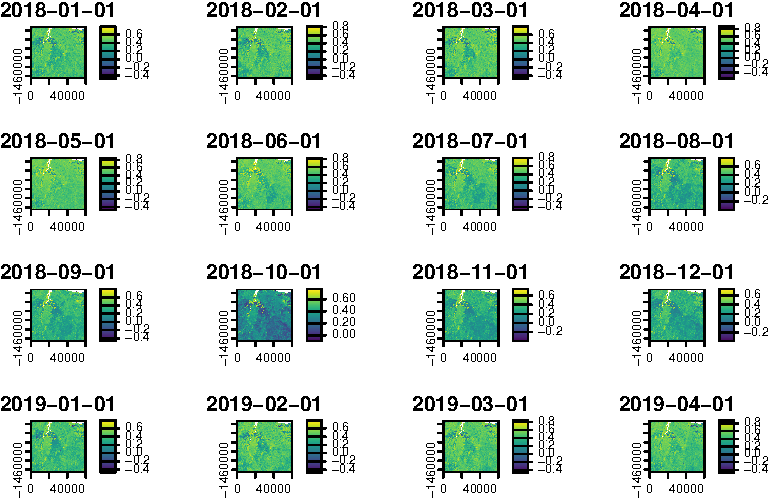
\includegraphics[keepaspectratio]{ssf_validation_files/figure-pdf/unnamed-chunk-2-1.pdf}}

\begin{Shaded}
\begin{Highlighting}[]
\FunctionTok{plot}\NormalTok{(slope)}
\end{Highlighting}
\end{Shaded}

\pandocbounded{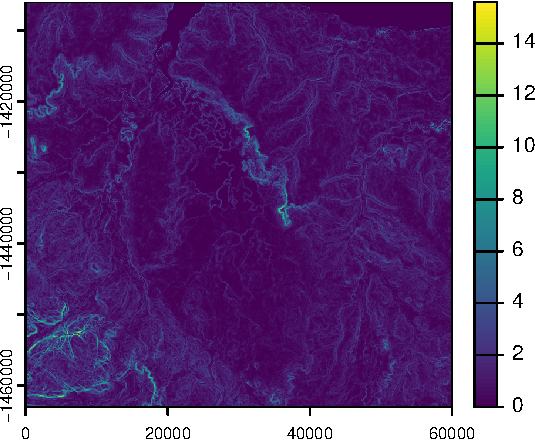
\includegraphics[keepaspectratio]{ssf_validation_files/figure-pdf/unnamed-chunk-2-2.pdf}}

\begin{Shaded}
\begin{Highlighting}[]
\FunctionTok{plot}\NormalTok{(veg\_herby)}
\end{Highlighting}
\end{Shaded}

\pandocbounded{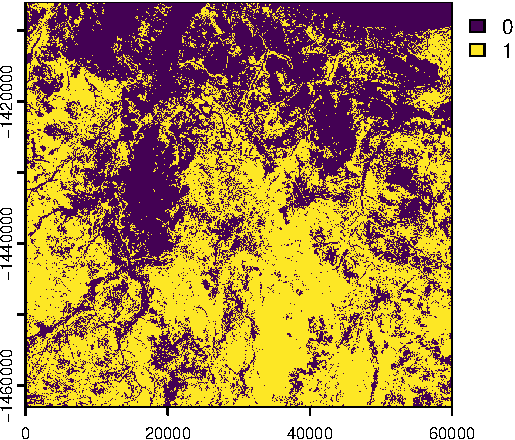
\includegraphics[keepaspectratio]{ssf_validation_files/figure-pdf/unnamed-chunk-2-3.pdf}}

\begin{Shaded}
\begin{Highlighting}[]
\FunctionTok{plot}\NormalTok{(canopy\_cover)}
\end{Highlighting}
\end{Shaded}

\pandocbounded{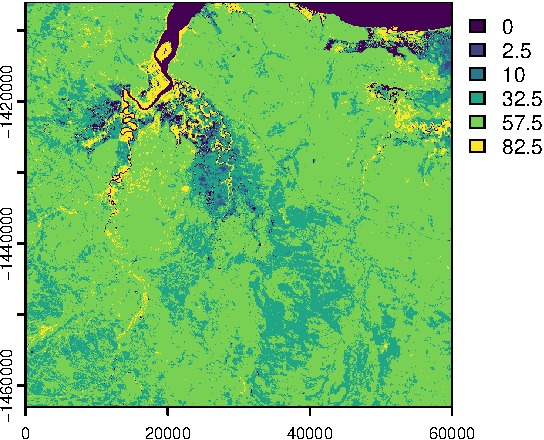
\includegraphics[keepaspectratio]{ssf_validation_files/figure-pdf/unnamed-chunk-2-4.pdf}}

\section{Generating the data to fit a deepSSF
model}\label{generating-the-data-to-fit-a-deepssf-model}

\subsection{Set up the spatial extent of the local
covariates}\label{set-up-the-spatial-extent-of-the-local-covariates}

\begin{Shaded}
\begin{Highlighting}[]
\CommentTok{\# get the resolution from the covariates}
\NormalTok{res }\OtherTok{\textless{}{-}}\NormalTok{ terra}\SpecialCharTok{::}\FunctionTok{res}\NormalTok{(ndvi\_projected)[}\DecValTok{1}\NormalTok{]}

\CommentTok{\# how much to trim on either side of the location, }
\CommentTok{\# this will determine the extent of the spatial inputs to the deepSSF model}
\NormalTok{buffer }\OtherTok{\textless{}{-}} \DecValTok{1250} \SpecialCharTok{+}\NormalTok{ (res}\SpecialCharTok{/}\DecValTok{2}\NormalTok{)}
\CommentTok{\# calculate the number of cells in each axis}
\NormalTok{nxn\_cells }\OtherTok{\textless{}{-}}\NormalTok{ buffer}\SpecialCharTok{*}\DecValTok{2}\SpecialCharTok{/}\NormalTok{res}

\CommentTok{\# hourly lag {-} to set larger time differences between locations}
\NormalTok{hourly\_lag }\OtherTok{\textless{}{-}} \DecValTok{1}
\end{Highlighting}
\end{Shaded}

\section{Evaluate next-step ahead
predictions}\label{evaluate-next-step-ahead-predictions}

\subsection{Create distance and bearing layers for the movement
probability}\label{create-distance-and-bearing-layers-for-the-movement-probability}

\begin{Shaded}
\begin{Highlighting}[]
\NormalTok{image\_dim }\OtherTok{\textless{}{-}} \DecValTok{101}
\NormalTok{pixel\_size }\OtherTok{\textless{}{-}} \DecValTok{25}
\NormalTok{center }\OtherTok{\textless{}{-}}\NormalTok{ image\_dim }\SpecialCharTok{\%/\%} \DecValTok{2}

\CommentTok{\# Create matrices of indices}
\NormalTok{x }\OtherTok{\textless{}{-}} \FunctionTok{matrix}\NormalTok{(}\FunctionTok{rep}\NormalTok{(}\DecValTok{0}\SpecialCharTok{:}\NormalTok{(image\_dim }\SpecialCharTok{{-}} \DecValTok{1}\NormalTok{), image\_dim), }\AttributeTok{nrow =}\NormalTok{ image\_dim, }\AttributeTok{byrow =} \ConstantTok{TRUE}\NormalTok{)}
\NormalTok{y }\OtherTok{\textless{}{-}} \FunctionTok{matrix}\NormalTok{(}\FunctionTok{rep}\NormalTok{(}\DecValTok{0}\SpecialCharTok{:}\NormalTok{(image\_dim }\SpecialCharTok{{-}} \DecValTok{1}\NormalTok{), }\AttributeTok{each =}\NormalTok{ image\_dim), }\AttributeTok{nrow =}\NormalTok{ image\_dim, }\AttributeTok{byrow =} \ConstantTok{TRUE}\NormalTok{)}

\CommentTok{\# Compute the distance layer}
\NormalTok{distance\_layer }\OtherTok{\textless{}{-}} \FunctionTok{sqrt}\NormalTok{((pixel\_size }\SpecialCharTok{*}\NormalTok{ (x }\SpecialCharTok{{-}}\NormalTok{ center))}\SpecialCharTok{\^{}}\DecValTok{2} \SpecialCharTok{+}\NormalTok{ (pixel\_size }\SpecialCharTok{*}\NormalTok{ (y }\SpecialCharTok{{-}}\NormalTok{ center))}\SpecialCharTok{\^{}}\DecValTok{2}\NormalTok{)}

\CommentTok{\# Change the center cell to the average distance from the center to the edge of the pixel}
\NormalTok{distance\_layer[center }\SpecialCharTok{+} \DecValTok{1}\NormalTok{, center }\SpecialCharTok{+} \DecValTok{1}\NormalTok{] }\OtherTok{\textless{}{-}} \FloatTok{0.56} \SpecialCharTok{*}\NormalTok{ pixel\_size}

\CommentTok{\# Compute the bearing layer}
\NormalTok{bearing\_layer }\OtherTok{\textless{}{-}} \FunctionTok{atan2}\NormalTok{(center }\SpecialCharTok{{-}}\NormalTok{ y, x }\SpecialCharTok{{-}}\NormalTok{ center)}

\CommentTok{\# Convert the distance and bearing matrices to raster layers}
\NormalTok{distance\_layer }\OtherTok{\textless{}{-}} \FunctionTok{rast}\NormalTok{(distance\_layer)}
\NormalTok{bearing\_layer }\OtherTok{\textless{}{-}} \FunctionTok{rast}\NormalTok{(bearing\_layer)}

\CommentTok{\# Optional: Plot the distance and bearing rasters}
\FunctionTok{plot}\NormalTok{(distance\_layer, }\AttributeTok{main =} \StringTok{"Distance from Center"}\NormalTok{)}
\end{Highlighting}
\end{Shaded}

\pandocbounded{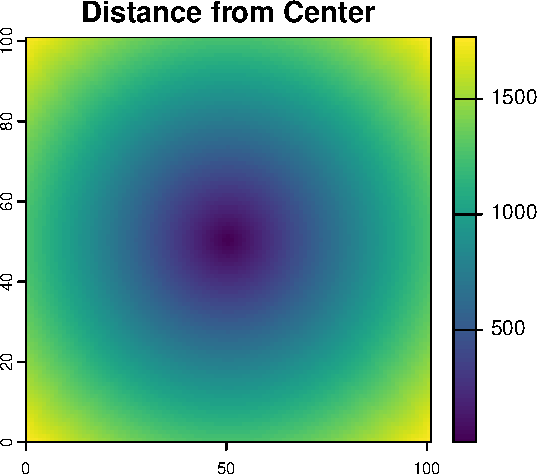
\includegraphics[keepaspectratio]{ssf_validation_files/figure-pdf/unnamed-chunk-4-1.pdf}}

\begin{Shaded}
\begin{Highlighting}[]
\FunctionTok{plot}\NormalTok{(bearing\_layer, }\AttributeTok{main =} \StringTok{"Bearing from Center"}\NormalTok{)}
\end{Highlighting}
\end{Shaded}

\pandocbounded{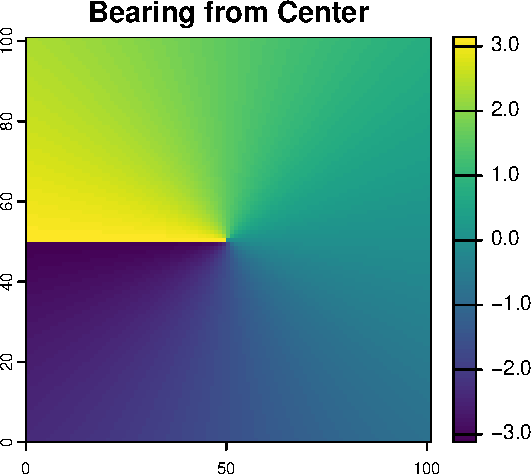
\includegraphics[keepaspectratio]{ssf_validation_files/figure-pdf/unnamed-chunk-4-2.pdf}}

\begin{Shaded}
\begin{Highlighting}[]
\NormalTok{distance\_values }\OtherTok{\textless{}{-}}\NormalTok{ terra}\SpecialCharTok{::}\FunctionTok{values}\NormalTok{(distance\_layer)}
\NormalTok{bearing\_values }\OtherTok{\textless{}{-}}\NormalTok{ terra}\SpecialCharTok{::}\FunctionTok{values}\NormalTok{(bearing\_layer)}
\end{Highlighting}
\end{Shaded}

\section{Calculating the habitat selection
probabilities}\label{calculating-the-habitat-selection-probabilities}

The habitat selection term of a step selection function is typically
modelled analogously to a resource-selection function (RSF), that
assumes an exponential (log-linear) form as

\[
    \omega(\mathbf{X}(s_t); \boldsymbol{\beta}(\tau; \boldsymbol{\alpha})) = \exp(\beta_{1}(\tau; \boldsymbol{\alpha}_1) X_1(s_t) + \cdots + \beta_{n}(\tau; \boldsymbol{\alpha}_n) X_n(s_t)),
\]

where
\(\boldsymbol{\beta}(\tau; \boldsymbol{\alpha}) = (\beta_{1}(\tau; \boldsymbol{\alpha}_1), \ldots, \beta_{n}(\tau; \boldsymbol{\alpha}_n))\)
in our case,

\[
\beta_i(\tau; \boldsymbol{\alpha}_i) = \alpha_{i,0} + \sum_{j = 1}^P \alpha_{i,j} \sin \left(\frac{2j \pi \tau}{T} \right) + \sum_{j = 1}^P \alpha_{i,j + P} \cos \left(\frac{2j \pi \tau}{T} \right),
\]

and \(\boldsymbol{\alpha}_i = (\alpha_{i, 0}, \dots, \alpha_{i, 2P})\),
where \(P\) is the number of pairs of harmonics, e.g.~for \(P = 2\), for
each covariate there would be two sine terms and two cosine terms, as
well as the linear term denoted by \(\alpha_{i, 0}\). The \(+ P\) term
in the \(\alpha\) index of the cosine term ensures that each
\(\alpha_i\) coefficient in \(\boldsymbol{\alpha}_i\) is unique.

To aid the computation of the simulations, we can precompute
\(\omega(\mathbf{X}(s_t); \boldsymbol{\beta}(\tau; \boldsymbol{\alpha}))\)
for each hour prior to running the simulations.

In the dataframe of temporally varying coefficients, for each covariate
we have reconstructed \(\beta_{i}(\tau; \boldsymbol{\alpha}_i)\) and
discretised for each hour of the day, resulting in \(\beta_{i,\tau}\)
for \(i = 1, \ldots, n\) where \(n\) is the number of covariates and
\(\tau = 1, \ldots, 24\).

Given these, we can solve
\(\omega(\mathbf{X}(s_t); \boldsymbol{\beta}(\tau; \boldsymbol{\alpha}))\)
for every hour of the day. This will result in an RSF map for each hour
of the day, which we will use in the simulations.

Then, when we do our step selection simulations, we can just subset
these maps by the current hour of the day, and extract the values of
\(\omega(\mathbf{X}(s_t); \boldsymbol{\beta}(\tau; \boldsymbol{\alpha}))\)
for each proposed step location, rather than solving
\(\omega(\mathbf{X}(s_t); \boldsymbol{\beta}(\tau; \boldsymbol{\alpha}))\)
for every step location.

\section{Calculating the next-step probabilities for the 0p and 2p
models}\label{calculating-the-next-step-probabilities-for-the-0p-and-2p-models}

\subsection{Select model coefficients}\label{select-model-coefficients}

\begin{Shaded}
\begin{Highlighting}[]
\NormalTok{model\_date }\OtherTok{\textless{}{-}} \StringTok{"2025{-}04{-}10"}
\NormalTok{focal\_id }\OtherTok{\textless{}{-}} \DecValTok{2005}
\end{Highlighting}
\end{Shaded}

\subsection{Setting up the data}\label{setting-up-the-data}

Read in the data of all individuals, which includes the focal or
`in-sample' individual that the model was fitted to, as well as the data
of the `out-of-sample' individuals that the model has never seen before,
and which is from quite a different environmental space (more on the
floodplain and closer to the river system).

\begin{Shaded}
\begin{Highlighting}[]
\CommentTok{\# create vector of GPS date filenames}
\NormalTok{buffalo\_data\_ids }\OtherTok{\textless{}{-}} \FunctionTok{list.files}\NormalTok{(}\AttributeTok{path =} \StringTok{"buffalo\_local\_data\_id"}\NormalTok{, }\AttributeTok{pattern =} \StringTok{".csv"}\NormalTok{) }
\FunctionTok{print}\NormalTok{(buffalo\_data\_ids)}
\end{Highlighting}
\end{Shaded}

\begin{verbatim}
 [1] "buffalo_2005_data_df_lag_1hr_n10297.csv"              
 [2] "buffalo_2014_data_df_lag_1hr_n6572.csv"               
 [3] "buffalo_2018_data_df_lag_1hr_n9440.csv"               
 [4] "buffalo_2021_data_df_lag_1hr_n6928.csv"               
 [5] "buffalo_2022_data_df_lag_1hr_n9099.csv"               
 [6] "buffalo_2024_data_df_lag_1hr_n9531.csv"               
 [7] "buffalo_2039_data_df_lag_1hr_n5569.csv"               
 [8] "buffalo_2154_data_df_lag_1hr_n10417.csv"              
 [9] "buffalo_2158_data_df_lag_1hr_n9700.csv"               
[10] "buffalo_2223_data_df_lag_1hr_n5310.csv"               
[11] "buffalo_2327_data_df_lag_1hr_n8983.csv"               
[12] "buffalo_2387_data_df_lag_1hr_n10409.csv"              
[13] "buffalo_2393_data_df_lag_1hr_n5299.csv"               
[14] "buffalo_temporal_cont_2005_data_df_lag_1hr_n10.csv"   
[15] "buffalo_temporal_cont_2005_data_df_lag_1hr_n100.csv"  
[16] "buffalo_temporal_cont_2005_data_df_lag_1hr_n10297.csv"
[17] "fixed_buffalo_2005_data_df_lag_1hr_n10297.csv"        
\end{verbatim}

\begin{Shaded}
\begin{Highlighting}[]
\NormalTok{ids }\OtherTok{\textless{}{-}} \FunctionTok{substr}\NormalTok{(buffalo\_data\_ids, }\DecValTok{9}\NormalTok{, }\DecValTok{12}\NormalTok{)}

\CommentTok{\# import data}
\NormalTok{buffalo\_id\_list }\OtherTok{\textless{}{-}} \FunctionTok{vector}\NormalTok{(}\AttributeTok{mode =} \StringTok{"list"}\NormalTok{, }\AttributeTok{length =} \FunctionTok{length}\NormalTok{(buffalo\_data\_ids))}

\CommentTok{\# read in the data}
\ControlFlowTok{for}\NormalTok{(i }\ControlFlowTok{in} \DecValTok{1}\SpecialCharTok{:}\FunctionTok{length}\NormalTok{(buffalo\_data\_ids))\{}
  
\NormalTok{  buffalo\_id\_list[[i]] }\OtherTok{\textless{}{-}}  \FunctionTok{read.csv}\NormalTok{(}\FunctionTok{paste}\NormalTok{(}\StringTok{"buffalo\_local\_data\_id/"}\NormalTok{,}
\NormalTok{                                             buffalo\_data\_ids[[i]], }
                                             \AttributeTok{sep =} \StringTok{""}\NormalTok{))}
\NormalTok{  buffalo\_id\_list[[i]]}\SpecialCharTok{$}\NormalTok{id }\OtherTok{\textless{}{-}}\NormalTok{ ids[i]}
  
\NormalTok{\}}
\end{Highlighting}
\end{Shaded}

\section{Calculating the next-step
probabilities}\label{calculating-the-next-step-probabilities}

This scrip takes a long time to run. As we have already calculated the
next-step probabilities for all individuals and all steps we will just
calculate a subset of the next-step predictions for illustration.

\begin{Shaded}
\begin{Highlighting}[]
\CommentTok{\# how many samples to illustrate the approach}
\NormalTok{n\_samples\_subset }\OtherTok{\textless{}{-}} \DecValTok{50}
\end{Highlighting}
\end{Shaded}

\subsection{Loop over all individuals and
models}\label{loop-over-all-individuals-and-models}

This script loops over all individuals and models, and calculates the
next-step probabilities for each step of the individual.

Here's high-level overview of the full chunk below

\subsubsection{\texorpdfstring{Outermost loop:
\texttt{for(k\ in\ 1:length(buffalo\_id\_list))\ \{...\}}}{Outermost loop: for(k in 1:length(buffalo\_id\_list)) \{...\}}}\label{outermost-loop-fork-in-1lengthbuffalo_id_list-...}

\begin{itemize}
\item
  \textbf{Data Preparation and Subsetting}

  \begin{itemize}
  \tightlist
  \item
    Each buffalo's trajectory (\texttt{data\_id}) is filtered to retain
    location steps within the local spatial spatial extent (±1250m).
  \item
    Any steps with missing data (e.g., turning angle, \texttt{ta}) are
    removed.
  \item
    The data is used to define a local bounding box
    (\texttt{template\_raster\_crop}) for cropping relevant raster
    datasets. This bounding box covers the extent of all points for that
    individual, and is for computational efficiency (so the full raster
    isn't being subsetted at every step). This is only done once per
    individual and is not the same as the local cropping done at every
    step.
  \end{itemize}
\item
  \textbf{Covariate Rasters Cropped to Bounding Box}

  \begin{itemize}
  \tightlist
  \item
    \textbf{NDVI} (Normalized Difference Vegetation Index - including
    squared term)
  \item
    \textbf{Canopy Cover} (including squared term)
  \item
    \textbf{Herbaceous Vegetation}
  \item
    \textbf{Slope}
  \end{itemize}
\end{itemize}

\subsubsection{\texorpdfstring{Middle loop:
\texttt{for(j\ in\ 1:length(model\_harmonics))\ \{...\}}}{Middle loop: for(j in 1:length(model\_harmonics)) \{...\}}}\label{middle-loop-forj-in-1lengthmodel_harmonics-...}

\begin{itemize}
\item
  \textbf{SSF Models}

  \begin{itemize}
  \tightlist
  \item
    The script selects one of the two models: \texttt{0p} (no temporal
    harmonics) or \texttt{2p} (temporal harmonics), indicated by
    \texttt{model\_harmonics}.
  \item
    Corresponding coefficients for each model are read from CSV files
    (e.g.,
    \texttt{"ssf\_coefficients/id\{focal\_id\}\_\{model\_harmonics{[}j{]}\}Daily\_coefs\_\{model\_date\}.csv"}).
  \item
    Only integer hours are used (filtered via
    \texttt{hour\ \%\%\ 1\ ==\ 0}).\\
  \end{itemize}
\end{itemize}

\subsubsection{\texorpdfstring{Inner loop:
\texttt{for\ (i\ in\ 2:n)\ \{..\}}}{Inner loop: for (i in 2:n) \{..\}}}\label{inner-loop-for-i-in-2n-..}

\begin{itemize}
\item
  \textbf{Loop Over Steps}\\
  For each step in the buffalo's trajectory:

  \begin{itemize}
  \item
    \textbf{Extract Local Covariates}\\
    A subset of each covariate raster is cropped to the step's spatial
    extent.
  \item
    \textbf{Habitat Selection Probability}

    \begin{itemize}
    \tightlist
    \item
      Relevant coefficients (e.g., \texttt{ndvi}, \texttt{ndvi\_2},
      \texttt{canopy}, \texttt{canopy\_2}, \texttt{herby},
      \texttt{slope}) for the current hour are retrieved, given the
      model.
    \item
      A log-probability (\texttt{habitat\_log}) is computed from the
      linear combination of covariates.
    \item
      The habitat selection probability is calculated by exponentiating
      the log-probability and normalising it to sum to 1.
    \end{itemize}
  \item
    \textbf{Movement Probability}

    \begin{itemize}
    \tightlist
    \item
      \textbf{Step length} is modeled via a Gamma distribution (using
      \texttt{shape} and \texttt{scale} parameters).
    \item
      \textbf{Turning angle} is modeled via the von Mises distribution
      (using \texttt{kappa} and a mean angle based on the previous
      step's bearing).
    \item
      The log-probability of these components is combined
      (\texttt{move\_log}) and normalised.
    \end{itemize}
  \item
    \textbf{Next-Step Probability}

    \begin{itemize}
    \tightlist
    \item
      The \textbf{habitat} and \textbf{movement} log-probabilities are
      summed to get the next-step log-probability.
    \item
      It is normalised to yield the \textbf{next-step probability} for
      each candidate pixel (where all pixels sum to 1).
    \item
      The script then extracts the probability at the buffalo's actual
      next location (\texttt{prob\_next\_step\_ssf\_0p} or
      \texttt{prob\_next\_step\_ssf\_2p}).
    \end{itemize}
  \end{itemize}
\end{itemize}

\subsubsection{\texorpdfstring{\textbf{Outputs}}{Outputs}}\label{outputs}

\begin{itemize}
\tightlist
\item
  For each step, the script appends probabilities
  (\texttt{prob\_habitat\_ssf\_0/2p},
  \texttt{prob\_movement\_ssf\_0/2p}, and
  \texttt{prob\_next\_step\_ssf\_0/2p}) to the data frame.
\end{itemize}

\subsubsection{\texorpdfstring{\textbf{Diagnostic
Plots}}{Diagnostic Plots}}\label{diagnostic-plots}

\begin{itemize}
\tightlist
\item
  For the first few steps of the first buffalo (which is the focal id),
  the script plots local covariate layers and the log-probability
  surfaces (habitat, movement, and combined next-step).
\end{itemize}

\begin{Shaded}
\begin{Highlighting}[]
\CommentTok{\#{-}{-}{-}{-}{-}{-}{-}{-}{-}{-}{-}{-}{-}{-}{-}{-}{-}{-}{-}{-}{-}{-}{-}{-}{-}{-}{-}{-}{-}{-}{-}{-}{-}{-}{-}{-}{-}{-}{-}{-}{-}{-}{-}{-}{-}{-}{-}{-}{-}{-}{-}{-}{-}{-}{-}{-}{-}{-}{-}{-}{-}{-}{-}{-}{-}{-}{-}{-}{-}{-}{-}{-}{-}}
\DocumentationTok{\#\#\# Select a buffalo\textquotesingle{}s data}
\CommentTok{\#{-}{-}{-}{-}{-}{-}{-}{-}{-}{-}{-}{-}{-}{-}{-}{-}{-}{-}{-}{-}{-}{-}{-}{-}{-}{-}{-}{-}{-}{-}{-}{-}{-}{-}{-}{-}{-}{-}{-}{-}{-}{-}{-}{-}{-}{-}{-}{-}{-}{-}{-}{-}{-}{-}{-}{-}{-}{-}{-}{-}{-}{-}{-}{-}{-}{-}{-}{-}{-}{-}{-}{-}{-}}

\CommentTok{\# for(k in 1:length(buffalo\_id\_list)) \{}

\ControlFlowTok{for}\NormalTok{(k }\ControlFlowTok{in} \DecValTok{1}\SpecialCharTok{:}\DecValTok{1}\NormalTok{) \{}

\NormalTok{  data\_id }\OtherTok{\textless{}{-}}\NormalTok{ buffalo\_id\_list[[k]]}
  \FunctionTok{attr}\NormalTok{(data\_id}\SpecialCharTok{$}\NormalTok{t\_, }\StringTok{"tzone"}\NormalTok{) }\OtherTok{\textless{}{-}} \StringTok{"Australia/Queensland"}
  \FunctionTok{attr}\NormalTok{(data\_id}\SpecialCharTok{$}\NormalTok{t2\_, }\StringTok{"tzone"}\NormalTok{) }\OtherTok{\textless{}{-}} \StringTok{"Australia/Queensland"}
  
\NormalTok{  data\_id }\OtherTok{\textless{}{-}}\NormalTok{ data\_id }\SpecialCharTok{\%\textgreater{}\%} \FunctionTok{mutate}\NormalTok{(}
    \AttributeTok{year\_t2 =} \FunctionTok{year}\NormalTok{(t2\_),}
    \AttributeTok{yday\_t2\_2018\_base =} \FunctionTok{ifelse}\NormalTok{(year\_t2 }\SpecialCharTok{==} \DecValTok{2018}\NormalTok{, yday\_t2, }\DecValTok{365}\SpecialCharTok{+}\NormalTok{yday\_t2)}
\NormalTok{  )}
  
\NormalTok{  sample\_extent }\OtherTok{\textless{}{-}} \DecValTok{1250}
  
  \CommentTok{\# remove steps that fall outside of the local spatial extent}
\NormalTok{  data\_id }\OtherTok{\textless{}{-}}\NormalTok{ data\_id }\SpecialCharTok{\%\textgreater{}\%}
    \FunctionTok{filter}\NormalTok{(x2\_cent }\SpecialCharTok{\textgreater{}} \SpecialCharTok{{-}}\NormalTok{sample\_extent }\SpecialCharTok{\&} 
\NormalTok{             x2\_cent }\SpecialCharTok{\textless{}}\NormalTok{ sample\_extent }\SpecialCharTok{\&} 
\NormalTok{             y2\_cent }\SpecialCharTok{\textgreater{}} \SpecialCharTok{{-}}\NormalTok{sample\_extent }\SpecialCharTok{\&} 
\NormalTok{             y2\_cent }\SpecialCharTok{\textless{}}\NormalTok{ sample\_extent) }\SpecialCharTok{\%\textgreater{}\%}
    \FunctionTok{drop\_na}\NormalTok{(ta)}
  
  \CommentTok{\# max(data\_id$yday\_t2\_2018\_base)}
  \CommentTok{\# write\_csv(data\_id, paste0("buffalo\_local\_data\_id/validation/validation\_", buffalo\_data\_ids[k]))}
  
  
\NormalTok{  model\_harmonics }\OtherTok{\textless{}{-}} \FunctionTok{c}\NormalTok{(}\StringTok{"0p"}\NormalTok{, }\StringTok{"2p"}\NormalTok{)}
  
\NormalTok{  test\_data }\OtherTok{\textless{}{-}}\NormalTok{ data\_id }\SpecialCharTok{\%\textgreater{}\%} \FunctionTok{slice}\NormalTok{(}\DecValTok{1}\SpecialCharTok{:}\DecValTok{100}\NormalTok{) }\CommentTok{\# test with a subset of the data}
  \CommentTok{\# test\_data \textless{}{-} data\_id}

  
  \CommentTok{\# subset rasters around all of the locations of the current buffalo (speeds up local subsetting)}
\NormalTok{  buffer }\OtherTok{\textless{}{-}} \DecValTok{2000}
\NormalTok{  template\_raster\_crop }\OtherTok{\textless{}{-}}\NormalTok{ terra}\SpecialCharTok{::}\FunctionTok{rast}\NormalTok{(}\AttributeTok{xmin =} \FunctionTok{min}\NormalTok{(test\_data}\SpecialCharTok{$}\NormalTok{x2\_) }\SpecialCharTok{{-}}\NormalTok{ buffer, }
                                      \AttributeTok{xmax =} \FunctionTok{max}\NormalTok{(test\_data}\SpecialCharTok{$}\NormalTok{x2\_) }\SpecialCharTok{+}\NormalTok{ buffer, }
                                      \AttributeTok{ymin =} \FunctionTok{min}\NormalTok{(test\_data}\SpecialCharTok{$}\NormalTok{y2\_) }\SpecialCharTok{{-}}\NormalTok{ buffer, }
                                      \AttributeTok{ymax =} \FunctionTok{max}\NormalTok{(test\_data}\SpecialCharTok{$}\NormalTok{y2\_) }\SpecialCharTok{+}\NormalTok{ buffer, }
                                      \AttributeTok{resolution =} \DecValTok{25}\NormalTok{, }
                                      \AttributeTok{crs =} \StringTok{"epsg:3112"}\NormalTok{)}
  
  \DocumentationTok{\#\# Crop the rasters}
\NormalTok{  ndvi\_projected\_cropped }\OtherTok{\textless{}{-}}\NormalTok{ terra}\SpecialCharTok{::}\FunctionTok{crop}\NormalTok{(ndvi\_projected, template\_raster\_crop)}
\NormalTok{  ndvi\_projected\_cropped\_sq }\OtherTok{\textless{}{-}}\NormalTok{ ndvi\_projected\_cropped}\SpecialCharTok{\^{}}\DecValTok{2}
  
\NormalTok{  canopy\_cover\_cropped }\OtherTok{\textless{}{-}}\NormalTok{ terra}\SpecialCharTok{::}\FunctionTok{crop}\NormalTok{(canopy\_cover, template\_raster\_crop)}
\NormalTok{  canopy01\_cropped }\OtherTok{\textless{}{-}}\NormalTok{ canopy\_cover\_cropped}\SpecialCharTok{/}\DecValTok{100}
\NormalTok{  canopy01\_cropped\_sq }\OtherTok{\textless{}{-}}\NormalTok{ canopy01\_cropped}\SpecialCharTok{\^{}}\DecValTok{2}
    
\NormalTok{  veg\_herby\_cropped }\OtherTok{\textless{}{-}}\NormalTok{ terra}\SpecialCharTok{::}\FunctionTok{crop}\NormalTok{(veg\_herby, template\_raster\_crop)}
\NormalTok{  slope\_cropped }\OtherTok{\textless{}{-}}\NormalTok{ terra}\SpecialCharTok{::}\FunctionTok{crop}\NormalTok{(slope, template\_raster\_crop)}
  
  \FunctionTok{tic}\NormalTok{()}
  
  \CommentTok{\#{-}{-}{-}{-}{-}{-}{-}{-}{-}{-}{-}{-}{-}{-}{-}{-}{-}{-}{-}{-}{-}{-}{-}{-}{-}{-}{-}{-}{-}{-}{-}{-}{-}{-}{-}{-}{-}{-}{-}{-}{-}{-}{-}{-}{-}{-}{-}{-}{-}{-}{-}{-}{-}{-}{-}{-}{-}{-}{-}{-}{-}{-}{-}{-}{-}{-}{-}{-}{-}{-}{-}{-}{-}}
  \DocumentationTok{\#\#\# Select a model (without temporal dynamics {-} 0p, or with temporal dynamics {-} 2p)}
  \CommentTok{\#{-}{-}{-}{-}{-}{-}{-}{-}{-}{-}{-}{-}{-}{-}{-}{-}{-}{-}{-}{-}{-}{-}{-}{-}{-}{-}{-}{-}{-}{-}{-}{-}{-}{-}{-}{-}{-}{-}{-}{-}{-}{-}{-}{-}{-}{-}{-}{-}{-}{-}{-}{-}{-}{-}{-}{-}{-}{-}{-}{-}{-}{-}{-}{-}{-}{-}{-}{-}{-}{-}{-}{-}{-}}
  
  \ControlFlowTok{for}\NormalTok{(j }\ControlFlowTok{in} \DecValTok{1}\SpecialCharTok{:}\FunctionTok{length}\NormalTok{(model\_harmonics)) \{}
  
\NormalTok{    ssf\_coefs\_file\_path }\OtherTok{\textless{}{-}} \FunctionTok{paste0}\NormalTok{(}\StringTok{"ssf\_coefficients/id"}\NormalTok{, focal\_id, }\StringTok{"\_"}\NormalTok{, model\_harmonics[j], }\StringTok{"Daily\_coefs\_80{-}10{-}10\_"}\NormalTok{, model\_date, }\StringTok{".csv"}\NormalTok{)}
    \FunctionTok{print}\NormalTok{(ssf\_coefs\_file\_path)}
    
\NormalTok{    ssf\_coefs }\OtherTok{\textless{}{-}} \FunctionTok{read\_csv}\NormalTok{(ssf\_coefs\_file\_path)}
    
    \CommentTok{\# keep only the integer hours using the modulo operator}
\NormalTok{    ssf\_coefs }\OtherTok{\textless{}{-}}\NormalTok{ ssf\_coefs }\SpecialCharTok{\%\textgreater{}\%} \FunctionTok{filter}\NormalTok{(ssf\_coefs}\SpecialCharTok{$}\NormalTok{hour }\SpecialCharTok{\%\%} \DecValTok{1} \SpecialCharTok{==} \DecValTok{0}\NormalTok{)}
    
    \CommentTok{\# for the progress bar {-} uncomment the line depending on if using subset}
    \CommentTok{\# for all data}
\NormalTok{    n }\OtherTok{\textless{}{-}} \FunctionTok{nrow}\NormalTok{(test\_data)}
    \CommentTok{\# for the subset}
    \CommentTok{\# n \textless{}{-} n\_samples\_subset}
    
\NormalTok{    pb }\OtherTok{\textless{}{-}}\NormalTok{ progress\_bar}\SpecialCharTok{$}\FunctionTok{new}\NormalTok{(}
      \AttributeTok{format =} \StringTok{"  Progress [:bar] :percent in :elapsed"}\NormalTok{,}
      \AttributeTok{total =}\NormalTok{ n,}
      \AttributeTok{clear =} \ConstantTok{FALSE}
\NormalTok{    )}
    
    
    \FunctionTok{tic}\NormalTok{()}
    
    \CommentTok{\#{-}{-}{-}{-}{-}{-}{-}{-}{-}{-}{-}{-}{-}{-}{-}{-}{-}{-}{-}{-}{-}{-}{-}{-}{-}{-}{-}{-}{-}{-}{-}{-}{-}{-}{-}{-}{-}{-}{-}{-}{-}{-}{-}{-}{-}{-}{-}{-}{-}{-}{-}{-}{-}{-}{-}{-}{-}{-}{-}{-}{-}{-}{-}{-}{-}{-}{-}{-}{-}{-}{-}{-}{-}}
    \DocumentationTok{\#\#\# Loop over every step in the trajectory}
    \CommentTok{\#{-}{-}{-}{-}{-}{-}{-}{-}{-}{-}{-}{-}{-}{-}{-}{-}{-}{-}{-}{-}{-}{-}{-}{-}{-}{-}{-}{-}{-}{-}{-}{-}{-}{-}{-}{-}{-}{-}{-}{-}{-}{-}{-}{-}{-}{-}{-}{-}{-}{-}{-}{-}{-}{-}{-}{-}{-}{-}{-}{-}{-}{-}{-}{-}{-}{-}{-}{-}{-}{-}{-}{-}{-}}
    
    \CommentTok{\# to calculate the next step probabilities for all samples}
    \CommentTok{\# for (i in 2:n) \{}
      
\NormalTok{    sample\_plot }\OtherTok{\textless{}{-}} \DecValTok{1}
      
    \ControlFlowTok{for}\NormalTok{ (i }\ControlFlowTok{in}\NormalTok{ sample\_plot}\SpecialCharTok{:}\NormalTok{(sample\_plot}\SpecialCharTok{+}\DecValTok{10}\NormalTok{)) \{}
    \CommentTok{\# for (i in sample\_plot:sample\_plot) \{}
    
    \CommentTok{\# for the subset}
    \CommentTok{\# for (i in 2:(n\_samples\_subset+1)) \{}
    
\NormalTok{      sample\_tm1 }\OtherTok{\textless{}{-}}\NormalTok{ test\_data[i}\DecValTok{{-}1}\NormalTok{, ] }\CommentTok{\# get the step at t {-} 1 for the bearing of the approaching step}
\NormalTok{      sample }\OtherTok{\textless{}{-}}\NormalTok{ test\_data[i, ]}
\NormalTok{      sample\_extent }\OtherTok{\textless{}{-}} \FunctionTok{ext}\NormalTok{(sample}\SpecialCharTok{$}\NormalTok{x\_min, sample}\SpecialCharTok{$}\NormalTok{x\_max, sample}\SpecialCharTok{$}\NormalTok{y\_min, sample}\SpecialCharTok{$}\NormalTok{y\_max)}
      
      
      \CommentTok{\#{-}{-}{-}{-}{-}{-}{-}{-}{-}{-}{-}{-}{-}{-}{-}{-}{-}{-}{-}{-}{-}{-}{-}{-}{-}{-}{-}{-}{-}{-}{-}{-}{-}{-}{-}{-}{-}{-}{-}{-}{-}{-}{-}{-}{-}{-}{-}{-}{-}{-}{-}{-}{-}{-}{-}{-}{-}{-}{-}{-}{-}{-}{-}{-}{-}{-}{-}{-}{-}{-}{-}{-}{-}}
      \DocumentationTok{\#\#\# Extract local covariates}
      \CommentTok{\#{-}{-}{-}{-}{-}{-}{-}{-}{-}{-}{-}{-}{-}{-}{-}{-}{-}{-}{-}{-}{-}{-}{-}{-}{-}{-}{-}{-}{-}{-}{-}{-}{-}{-}{-}{-}{-}{-}{-}{-}{-}{-}{-}{-}{-}{-}{-}{-}{-}{-}{-}{-}{-}{-}{-}{-}{-}{-}{-}{-}{-}{-}{-}{-}{-}{-}{-}{-}{-}{-}{-}{-}{-}}
      \CommentTok{\# NDVI}
\NormalTok{      ndvi\_index }\OtherTok{\textless{}{-}} \FunctionTok{which.min}\NormalTok{(}\FunctionTok{abs}\NormalTok{(}\FunctionTok{difftime}\NormalTok{(sample}\SpecialCharTok{$}\NormalTok{t\_, terra}\SpecialCharTok{::}\FunctionTok{time}\NormalTok{(ndvi\_projected\_cropped))))}
\NormalTok{      ndvi\_sample }\OtherTok{\textless{}{-}} \FunctionTok{crop}\NormalTok{(ndvi\_projected[[ndvi\_index]], sample\_extent)}
      \CommentTok{\# NDVI \^{} 2}
\NormalTok{      ndvi\_sq\_sample }\OtherTok{\textless{}{-}} \FunctionTok{crop}\NormalTok{(ndvi\_projected\_cropped\_sq[[ndvi\_index]], sample\_extent)}
      \CommentTok{\# Canopy cover}
\NormalTok{      canopy\_sample }\OtherTok{\textless{}{-}} \FunctionTok{crop}\NormalTok{(canopy01\_cropped, sample\_extent)}
      \CommentTok{\# Canopy cover \^{} 2}
\NormalTok{      canopy\_sq\_sample }\OtherTok{\textless{}{-}} \FunctionTok{crop}\NormalTok{(canopy01\_cropped\_sq, sample\_extent)}
      \CommentTok{\# Herbaceous vegetation}
\NormalTok{      veg\_herby\_sample }\OtherTok{\textless{}{-}} \FunctionTok{crop}\NormalTok{(veg\_herby\_cropped, sample\_extent)}
      \CommentTok{\# Slope}
\NormalTok{      slope\_sample }\OtherTok{\textless{}{-}} \FunctionTok{crop}\NormalTok{(slope\_cropped, sample\_extent)}
      
      \CommentTok{\# create a SpatVector from the coordinates}
\NormalTok{      next\_step\_vect }\OtherTok{\textless{}{-}} \FunctionTok{vect}\NormalTok{(}\FunctionTok{cbind}\NormalTok{(sample}\SpecialCharTok{$}\NormalTok{x2\_, sample}\SpecialCharTok{$}\NormalTok{y2\_), }\AttributeTok{crs =} \FunctionTok{crs}\NormalTok{(ndvi\_sample))}
      
      
      \CommentTok{\#{-}{-}{-}{-}{-}{-}{-}{-}{-}{-}{-}{-}{-}{-}{-}{-}{-}{-}{-}{-}{-}{-}{-}{-}{-}{-}{-}{-}{-}{-}{-}{-}{-}{-}{-}{-}{-}{-}{-}{-}{-}{-}{-}{-}{-}{-}{-}{-}{-}{-}{-}{-}{-}{-}{-}{-}{-}{-}{-}{-}{-}{-}{-}{-}{-}{-}{-}{-}{-}{-}{-}{-}{-}}
      \DocumentationTok{\#\#\# calculate the next{-}step probability surfaces}
      \CommentTok{\#{-}{-}{-}{-}{-}{-}{-}{-}{-}{-}{-}{-}{-}{-}{-}{-}{-}{-}{-}{-}{-}{-}{-}{-}{-}{-}{-}{-}{-}{-}{-}{-}{-}{-}{-}{-}{-}{-}{-}{-}{-}{-}{-}{-}{-}{-}{-}{-}{-}{-}{-}{-}{-}{-}{-}{-}{-}{-}{-}{-}{-}{-}{-}{-}{-}{-}{-}{-}{-}{-}{-}{-}{-}}
      
      
      \DocumentationTok{\#\#\# Habitat selection probability}
      \CommentTok{\#{-}{-}{-}{-}{-}{-}{-}{-}{-}{-}{-}{-}{-}{-}{-}{-}{-}{-}{-}{-}{-}{-}{-}{-}{-}{-}{-}{-}{-}{-}{-}{-}{-}{-}{-}{-}{-}{-}{-}{-}{-}{-}{-}{-}{-}{-}{-}{-}{-}{-}{-}{-}{-}{-}{-}{-}{-}{-}{-}{-}{-}{-}{-}{-}{-}{-}{-}{-}{-}{-}{-}{-}{-}}
      
      \CommentTok{\# get the coefficients for the appropriate hour}
\NormalTok{      coef\_hour }\OtherTok{\textless{}{-}} \FunctionTok{which}\NormalTok{(ssf\_coefs}\SpecialCharTok{$}\NormalTok{hour }\SpecialCharTok{==}\NormalTok{ sample}\SpecialCharTok{$}\NormalTok{hour\_t2)}
      
      \CommentTok{\# multiply covariate values by coefficients}
      \CommentTok{\# ndvi}
\NormalTok{      ndvi\_linear }\OtherTok{\textless{}{-}}\NormalTok{ ndvi\_sample }\SpecialCharTok{*}\NormalTok{ ssf\_coefs}\SpecialCharTok{$}\NormalTok{ndvi[[coef\_hour]]}
\NormalTok{      ndvi\_quad }\OtherTok{\textless{}{-}}\NormalTok{ ndvi\_sq\_sample }\SpecialCharTok{*}\NormalTok{ ssf\_coefs}\SpecialCharTok{$}\NormalTok{ndvi\_2[[coef\_hour]]}
      \CommentTok{\# canopy cover}
\NormalTok{      canopy\_linear }\OtherTok{\textless{}{-}}\NormalTok{ canopy\_sample }\SpecialCharTok{*}\NormalTok{ ssf\_coefs}\SpecialCharTok{$}\NormalTok{canopy[[coef\_hour]]}
\NormalTok{      canopy\_quad }\OtherTok{\textless{}{-}}\NormalTok{ canopy\_sq\_sample }\SpecialCharTok{*}\NormalTok{ ssf\_coefs}\SpecialCharTok{$}\NormalTok{canopy\_2[[coef\_hour]]}
      \CommentTok{\# veg\_herby}
\NormalTok{      veg\_herby\_pred }\OtherTok{\textless{}{-}}\NormalTok{ veg\_herby\_sample }\SpecialCharTok{*}\NormalTok{ ssf\_coefs}\SpecialCharTok{$}\NormalTok{herby[[coef\_hour]]}
      \CommentTok{\# slope}
\NormalTok{      slope\_pred }\OtherTok{\textless{}{-}}\NormalTok{ slope\_sample }\SpecialCharTok{*}\NormalTok{ ssf\_coefs}\SpecialCharTok{$}\NormalTok{slope[[coef\_hour]]}
      
      \CommentTok{\# combining all covariates (on the log{-}scale)}
\NormalTok{      habitat\_log }\OtherTok{\textless{}{-}}\NormalTok{ ndvi\_linear }\SpecialCharTok{+}\NormalTok{ ndvi\_quad }\SpecialCharTok{+}\NormalTok{ canopy\_linear }\SpecialCharTok{+}\NormalTok{ canopy\_quad }\SpecialCharTok{+}\NormalTok{ slope\_pred }\SpecialCharTok{+}\NormalTok{ veg\_herby\_pred}
      
      \CommentTok{\# create template raster}
\NormalTok{      habitat\_pred }\OtherTok{\textless{}{-}}\NormalTok{ habitat\_log}
      \CommentTok{\# convert to normalised probability}
\NormalTok{      habitat\_pred[] }\OtherTok{\textless{}{-}} \FunctionTok{exp}\NormalTok{(}\FunctionTok{values}\NormalTok{(habitat\_log) }\SpecialCharTok{{-}} \FunctionTok{max}\NormalTok{(}\FunctionTok{values}\NormalTok{(habitat\_log), }\AttributeTok{na.rm =}\NormalTok{ T)) }\SpecialCharTok{/} 
        \FunctionTok{sum}\NormalTok{(}\FunctionTok{exp}\NormalTok{(}\FunctionTok{values}\NormalTok{(habitat\_log) }\SpecialCharTok{{-}} \FunctionTok{max}\NormalTok{(}\FunctionTok{values}\NormalTok{(habitat\_log), }\AttributeTok{na.rm =}\NormalTok{ T)), }\AttributeTok{na.rm =}\NormalTok{ T)}
      \CommentTok{\# print(sum(values(habitat\_pred)))}
      
      \CommentTok{\# habitat probability value at the next step}
\NormalTok{      prob\_habitat }\OtherTok{\textless{}{-}} \FunctionTok{as.numeric}\NormalTok{(terra}\SpecialCharTok{::}\FunctionTok{extract}\NormalTok{(habitat\_pred, next\_step\_vect)[}\DecValTok{2}\NormalTok{])}
      \CommentTok{\# print(paste0("Habitat probability: ", prob\_habitat))}
      
      
      \DocumentationTok{\#\#\# Movement Probability}
      \CommentTok{\#{-}{-}{-}{-}{-}{-}{-}{-}{-}{-}{-}{-}{-}{-}{-}{-}{-}{-}{-}{-}{-}{-}{-}{-}{-}{-}{-}{-}{-}{-}{-}{-}{-}{-}{-}{-}{-}{-}{-}{-}{-}{-}{-}{-}{-}{-}{-}{-}{-}{-}{-}{-}{-}{-}{-}{-}{-}{-}{-}{-}{-}{-}{-}{-}{-}{-}{-}{-}{-}{-}{-}{-}{-}}
      
      \CommentTok{\# step lengths}
      \CommentTok{\# calculated on the log scale}
      \CommentTok{\# subtract the log(distance values to account for the change in movement variables {-} Appendix in paper)}
\NormalTok{      step\_log }\OtherTok{\textless{}{-}}\NormalTok{ habitat\_log}
\NormalTok{      step\_log[] }\OtherTok{\textless{}{-}} \FunctionTok{dgamma}\NormalTok{(distance\_values, }
                           \AttributeTok{shape =}\NormalTok{ ssf\_coefs}\SpecialCharTok{$}\NormalTok{shape[[coef\_hour]], }
                           \AttributeTok{scale =}\NormalTok{ ssf\_coefs}\SpecialCharTok{$}\NormalTok{scale[[coef\_hour]], }\AttributeTok{log =} \ConstantTok{TRUE}\NormalTok{) }\SpecialCharTok{{-}} \FunctionTok{log}\NormalTok{(distance\_values)}
      
      \CommentTok{\# normalise the step length probabilities}
      \CommentTok{\# step\_log[] \textless{}{-} values(step\_log) {-} max(values(step\_log), na.rm = T) {-} }
      \CommentTok{\#   log(sum(exp(values(step\_log) {-} max(values(step\_log), na.rm = T))))}
      
      \CommentTok{\# check that they sum to 1}
      \CommentTok{\# print(sum(exp(values(step\_log))))}
            
      
      \CommentTok{\# turning angles}
\NormalTok{      ta\_log }\OtherTok{\textless{}{-}}\NormalTok{ habitat\_log}
\NormalTok{      vm\_mu }\OtherTok{\textless{}{-}}\NormalTok{ sample}\SpecialCharTok{$}\NormalTok{bearing}
\NormalTok{      vm\_mu\_updated }\OtherTok{\textless{}{-}} \FunctionTok{ifelse}\NormalTok{(ssf\_coefs}\SpecialCharTok{$}\NormalTok{kappa[[coef\_hour]] }\SpecialCharTok{\textgreater{}} \DecValTok{0}\NormalTok{, sample\_tm1}\SpecialCharTok{$}\NormalTok{bearing, sample\_tm1}\SpecialCharTok{$}\NormalTok{bearing }\SpecialCharTok{{-}}\NormalTok{ pi)}
\NormalTok{      ta\_log[] }\OtherTok{\textless{}{-}} \FunctionTok{suppressWarnings}\NormalTok{(circular}\SpecialCharTok{::}\FunctionTok{dvonmises}\NormalTok{(bearing\_values, }
                                                       \AttributeTok{mu =}\NormalTok{ vm\_mu\_updated, }
                                                       \AttributeTok{kappa =} \FunctionTok{abs}\NormalTok{(ssf\_coefs}\SpecialCharTok{$}\NormalTok{kappa[[coef\_hour]]), }
                                                       \AttributeTok{log =} \ConstantTok{TRUE}\NormalTok{))}
      
      \CommentTok{\# normalise the turning angle probabilities}
      \CommentTok{\# ta\_log[] \textless{}{-} values(ta\_log) {-} max(values(ta\_log), na.rm = T) {-} }
      \CommentTok{\#   log(sum(exp(values(ta\_log) {-} max(values(ta\_log), na.rm = T))))}
      
      \CommentTok{\# check that they sum to 1}
      \CommentTok{\# print(sum(exp(values(ta\_log))))}
      
      \CommentTok{\# combine the step and turning angle probabilities}
\NormalTok{      move\_log }\OtherTok{\textless{}{-}}\NormalTok{ step\_log }\SpecialCharTok{+}\NormalTok{ ta\_log}
      
      \CommentTok{\# create template raster}
\NormalTok{      move\_pred }\OtherTok{\textless{}{-}}\NormalTok{ habitat\_log}
      \CommentTok{\# convert to normalised probability}
\NormalTok{      move\_pred[] }\OtherTok{\textless{}{-}} \FunctionTok{exp}\NormalTok{(}\FunctionTok{values}\NormalTok{(move\_log) }\SpecialCharTok{{-}} \FunctionTok{max}\NormalTok{(}\FunctionTok{values}\NormalTok{(move\_log), }\AttributeTok{na.rm =}\NormalTok{ T)) }\SpecialCharTok{/} 
        \FunctionTok{sum}\NormalTok{(}\FunctionTok{exp}\NormalTok{(}\FunctionTok{values}\NormalTok{(move\_log) }\SpecialCharTok{{-}} \FunctionTok{max}\NormalTok{(}\FunctionTok{values}\NormalTok{(move\_log), }\AttributeTok{na.rm =}\NormalTok{ T)), }\AttributeTok{na.rm =}\NormalTok{ T)}
      \CommentTok{\# print(sum(values(move\_pred)))}
      
      \CommentTok{\# movement probability value at the next step}
\NormalTok{      prob\_movement }\OtherTok{\textless{}{-}} \FunctionTok{as.numeric}\NormalTok{(terra}\SpecialCharTok{::}\FunctionTok{extract}\NormalTok{(move\_pred, next\_step\_vect)[}\DecValTok{2}\NormalTok{])}
      \CommentTok{\# print(prob\_movement)}
      
      
      \CommentTok{\# Next{-}step probability}
      \CommentTok{\#{-}{-}{-}{-}{-}{-}{-}{-}{-}{-}{-}{-}{-}{-}{-}{-}{-}{-}{-}{-}{-}{-}{-}{-}{-}{-}{-}{-}{-}{-}{-}{-}{-}{-}{-}{-}{-}{-}{-}{-}{-}{-}{-}{-}{-}{-}{-}{-}{-}{-}{-}{-}{-}{-}{-}{-}{-}{-}{-}{-}{-}{-}{-}{-}{-}{-}{-}{-}{-}{-}{-}{-}{-}}
      
      \CommentTok{\# calculate the next{-}step log probability}
\NormalTok{      next\_step\_log }\OtherTok{\textless{}{-}}\NormalTok{ habitat\_log }\SpecialCharTok{+}\NormalTok{ move\_log}
      
      \CommentTok{\# create template raster}
\NormalTok{      next\_step\_pred }\OtherTok{\textless{}{-}}\NormalTok{ habitat\_log}
      \CommentTok{\# normalise using log{-}sum{-}exp trick}
\NormalTok{      next\_step\_pred[] }\OtherTok{\textless{}{-}} \FunctionTok{exp}\NormalTok{(}\FunctionTok{values}\NormalTok{(next\_step\_log) }\SpecialCharTok{{-}} \FunctionTok{max}\NormalTok{(}\FunctionTok{values}\NormalTok{(next\_step\_log), }\AttributeTok{na.rm =}\NormalTok{ T)) }\SpecialCharTok{/} 
        \FunctionTok{sum}\NormalTok{(}\FunctionTok{exp}\NormalTok{(}\FunctionTok{values}\NormalTok{(next\_step\_log) }\SpecialCharTok{{-}} \FunctionTok{max}\NormalTok{(}\FunctionTok{values}\NormalTok{(next\_step\_log), }\AttributeTok{na.rm =}\NormalTok{ T)), }\AttributeTok{na.rm =}\NormalTok{ T)}
      \CommentTok{\# print(sum(values(next\_step\_pred)))}
      
      \CommentTok{\# check next{-}step location}
\NormalTok{      next\_step\_sample }\OtherTok{\textless{}{-}}\NormalTok{ terra}\SpecialCharTok{::}\FunctionTok{mask}\NormalTok{(next\_step\_pred, next\_step\_vect, }\AttributeTok{inverse =}\NormalTok{ T)}
      \CommentTok{\# plot(next\_step\_sample)}
      
      \CommentTok{\# check which cell is NA in rows and columns}
      \CommentTok{\# print(rowColFromCell(next\_step\_pred, which(is.na(values(next\_step\_sample)))))}
      
      \CommentTok{\# NDVI value at next step (to check against the deepSSF version)}
      \CommentTok{\# ndvi\_next\_step \textless{}{-} as.numeric(terra::extract(ndvi\_sample, next\_step\_vect)[2])}
      \CommentTok{\# print(paste("NDVI value = ", ndvi\_next\_step))}
      
      \CommentTok{\# next{-}step probability value at the next step}
\NormalTok{      prob\_next\_step }\OtherTok{\textless{}{-}} \FunctionTok{as.numeric}\NormalTok{(terra}\SpecialCharTok{::}\FunctionTok{extract}\NormalTok{(next\_step\_pred, next\_step\_vect)[}\DecValTok{2}\NormalTok{])}
      \CommentTok{\# print(prob\_next\_step)}
      
\NormalTok{      test\_data[i, }\FunctionTok{paste0}\NormalTok{(}\StringTok{"prob\_habitat\_ssf\_"}\NormalTok{, model\_harmonics[j])] }\OtherTok{\textless{}{-}}\NormalTok{ prob\_habitat}
\NormalTok{      test\_data[i, }\FunctionTok{paste0}\NormalTok{(}\StringTok{"prob\_movement\_ssf\_"}\NormalTok{, model\_harmonics[j])] }\OtherTok{\textless{}{-}}\NormalTok{ prob\_movement}
\NormalTok{      test\_data[i, }\FunctionTok{paste0}\NormalTok{(}\StringTok{"prob\_next\_step\_ssf\_"}\NormalTok{, model\_harmonics[j])] }\OtherTok{\textless{}{-}}\NormalTok{ prob\_next\_step}
      
      \CommentTok{\# plot a few local covariates and the predictions for the focal buffalo}
      \CommentTok{\# if(k == 1 \& i \textless{} 7)\{}
      \ControlFlowTok{if}\NormalTok{(k }\SpecialCharTok{==} \DecValTok{1}\NormalTok{)\{}
        
        \FunctionTok{print}\NormalTok{(sample)}
        
        \FunctionTok{png}\NormalTok{(}\FunctionTok{paste0}\NormalTok{(}\StringTok{"outputs/next\_step\_validation/ndvi\_step\_"}\NormalTok{, i, }\StringTok{".png"}\NormalTok{),}
        \AttributeTok{width =} \DecValTok{800}\NormalTok{, }\AttributeTok{height =} \DecValTok{750}\NormalTok{, }\AttributeTok{res =} \DecValTok{150}\NormalTok{)}
        \FunctionTok{plot}\NormalTok{(ndvi\_sample, }\AttributeTok{main =} \StringTok{"NDVI"}\NormalTok{)}
        \FunctionTok{dev.off}\NormalTok{()}
        
        \FunctionTok{png}\NormalTok{(}\FunctionTok{paste0}\NormalTok{(}\StringTok{"outputs/next\_step\_validation/canopy\_"}\NormalTok{, i, }\StringTok{".png"}\NormalTok{),}
        \AttributeTok{width =} \DecValTok{800}\NormalTok{, }\AttributeTok{height =} \DecValTok{750}\NormalTok{, }\AttributeTok{res =} \DecValTok{150}\NormalTok{)}
        \FunctionTok{plot}\NormalTok{(canopy\_sample, }\AttributeTok{main =} \StringTok{"Canopy cover"}\NormalTok{)}
        \FunctionTok{dev.off}\NormalTok{()}
        
        \FunctionTok{png}\NormalTok{(}\FunctionTok{paste0}\NormalTok{(}\StringTok{"outputs/next\_step\_validation/herby\_"}\NormalTok{, i, }\StringTok{".png"}\NormalTok{),}
        \AttributeTok{width =} \DecValTok{800}\NormalTok{, }\AttributeTok{height =} \DecValTok{750}\NormalTok{, }\AttributeTok{res =} \DecValTok{150}\NormalTok{)}
        \FunctionTok{plot}\NormalTok{(veg\_herby\_sample, }\AttributeTok{main =} \StringTok{"Herbaceous vegetation"}\NormalTok{)}
        \FunctionTok{dev.off}\NormalTok{()}
        
        \FunctionTok{png}\NormalTok{(}\FunctionTok{paste0}\NormalTok{(}\StringTok{"outputs/next\_step\_validation/slope\_"}\NormalTok{, i, }\StringTok{".png"}\NormalTok{),}
        \AttributeTok{width =} \DecValTok{800}\NormalTok{, }\AttributeTok{height =} \DecValTok{750}\NormalTok{, }\AttributeTok{res =} \DecValTok{150}\NormalTok{)}
        \FunctionTok{plot}\NormalTok{(slope\_sample, }\AttributeTok{main =} \StringTok{"Slope"}\NormalTok{)}
        \FunctionTok{dev.off}\NormalTok{()}
        
        
        \FunctionTok{png}\NormalTok{(}\FunctionTok{paste0}\NormalTok{(}\StringTok{"outputs/next\_step\_validation/habitat\_log\_step\_"}\NormalTok{, i, }\StringTok{"\_model\_"}\NormalTok{, j, }\StringTok{".png"}\NormalTok{),}
        \AttributeTok{width =} \DecValTok{800}\NormalTok{, }\AttributeTok{height =} \DecValTok{750}\NormalTok{, }\AttributeTok{res =} \DecValTok{150}\NormalTok{)}
        \FunctionTok{plot}\NormalTok{(terra}\SpecialCharTok{::}\FunctionTok{mask}\NormalTok{(}\FunctionTok{log}\NormalTok{(habitat\_pred), next\_step\_vect, }\AttributeTok{inverse =}\NormalTok{ T), }
             \AttributeTok{main =} \FunctionTok{paste0}\NormalTok{(}\StringTok{"Habitat selection (log) {-} Model "}\NormalTok{, model\_harmonics[j]))}
        \CommentTok{\# plot(habitat\_pred)}
        \FunctionTok{dev.off}\NormalTok{()}
        
        \FunctionTok{png}\NormalTok{(}\FunctionTok{paste0}\NormalTok{(}\StringTok{"outputs/next\_step\_validation/habitat\_step\_"}\NormalTok{, i, }\StringTok{"\_model\_"}\NormalTok{, j, }\StringTok{".png"}\NormalTok{),}
        \AttributeTok{width =} \DecValTok{800}\NormalTok{, }\AttributeTok{height =} \DecValTok{750}\NormalTok{, }\AttributeTok{res =} \DecValTok{150}\NormalTok{)}
        \FunctionTok{plot}\NormalTok{(terra}\SpecialCharTok{::}\FunctionTok{mask}\NormalTok{(habitat\_pred, next\_step\_vect, }\AttributeTok{inverse =}\NormalTok{ T), }
             \AttributeTok{main =} \FunctionTok{paste0}\NormalTok{(}\StringTok{"Habitat selection {-} Model "}\NormalTok{, model\_harmonics[j]))}
        \FunctionTok{dev.off}\NormalTok{()}
        
        \CommentTok{\# plot(step\_log, main = "")}
        \CommentTok{\# plot(ta\_log, main = "")}
        \FunctionTok{plot}\NormalTok{(terra}\SpecialCharTok{::}\FunctionTok{mask}\NormalTok{(}\FunctionTok{log}\NormalTok{(move\_pred), next\_step\_vect, }\AttributeTok{inverse =}\NormalTok{ T), }
             \AttributeTok{main =} \FunctionTok{paste0}\NormalTok{(}\StringTok{"Movement log{-}probability {-} Model "}\NormalTok{, model\_harmonics[j]))}
        \CommentTok{\# plot(move\_pred)}
        
        \FunctionTok{plot}\NormalTok{(terra}\SpecialCharTok{::}\FunctionTok{mask}\NormalTok{(}\FunctionTok{log}\NormalTok{(next\_step\_pred), next\_step\_vect, }\AttributeTok{inverse =}\NormalTok{ T), }
             \AttributeTok{main =} \FunctionTok{paste0}\NormalTok{(}\StringTok{"Next{-}step log{-}probability {-} Model "}\NormalTok{, model\_harmonics[j]))}
        \CommentTok{\# plot(next\_step\_pred)}
        
\NormalTok{      \}}
      
\NormalTok{      pb}\SpecialCharTok{$}\FunctionTok{tick}\NormalTok{()  }\CommentTok{\# Update progress bar}
       
\NormalTok{      \}}
    
    \FunctionTok{toc}\NormalTok{()}
    
\NormalTok{  \}}
  
  \CommentTok{\# write.csv(test\_data, file = paste0("outputs/next\_step\_validation/next\_step\_probs\_ssf\_80{-}10{-}10\_id", ids[k], "\_n\_samples", n, "\_", Sys.Date(), ".csv"))}
  
  \FunctionTok{gc}\NormalTok{()}
  
\NormalTok{\}}
\end{Highlighting}
\end{Shaded}

\begin{verbatim}
[1] "ssf_coefficients/id2005_0pDaily_coefs_80-10-10_2025-04-10.csv"
\end{verbatim}

\begin{verbatim}
Rows: 240 Columns: 13
-- Column specification --------------------------------------------------------
Delimiter: ","
dbl (13): hour, ndvi, ndvi_2, canopy, canopy_2, slope, herby, sl, log_sl, co...

i Use `spec()` to retrieve the full column specification for this data.
i Specify the column types or set `show_col_types = FALSE` to quiet this message.
\end{verbatim}

\begin{verbatim}
Warning in max(values(move_log), na.rm = T): no non-missing arguments to max;
returning -Inf
Warning in max(values(move_log), na.rm = T): no non-missing arguments to max;
returning -Inf
\end{verbatim}

\begin{verbatim}
Warning in max(values(next_step_log), na.rm = T): no non-missing arguments to
max; returning -Inf
Warning in max(values(next_step_log), na.rm = T): no non-missing arguments to
max; returning -Inf
\end{verbatim}

\begin{verbatim}
Warning: Failed to compute min/max, no valid pixels found in sampling. (GDAL
error 1)
\end{verbatim}

\begin{verbatim}
        x_       y_                   t_   id      x1_      y1_      x2_
1 41969.31 -1435671 2018-07-25T01:04:23Z 2005 41969.31 -1435671 41921.52
       y2_   x2_cent  y2_cent                  t2_ t_diff hour_t1 yday_t1
1 -1435654 -47.78894 16.85711 2018-07-25T02:04:39Z      1      11     206
  hour_t2  hour_t2_sin hour_t2_cos yday_t2 yday_t2_sin yday_t2_cos       sl
1      12 1.224606e-16          -1     206  -0.3913578  -0.9202386 50.67489
    log_sl  bearing bearing_sin bearing_cos       ta   cos_ta    x_min    x_max
1 3.925431 2.802478   0.3326521  -0.9430496 1.367942 0.201466 40706.81 43231.81
     y_min    y_max s2_index points_vect_cent year_t2 yday_t2_2018_base
1 -1436934 -1434409        7               NA    2018               206
\end{verbatim}

\begin{verbatim}
Warning: Failed to compute min/max, no valid pixels found in sampling. (GDAL
error 1)
\end{verbatim}

\pandocbounded{
\includegraphics[keepaspectratio]{ssf_validation_files/figure-pdf/unnamed-chunk-8-1.pdf}}

\begin{verbatim}
Warning: Failed to compute min/max, no valid pixels found in sampling. (GDAL
error 1)
\end{verbatim}

\begin{verbatim}
        x_       y_                   t_   id      x1_      y1_      x2_
2 41921.52 -1435654 2018-07-25T02:04:39Z 2005 41921.52 -1435654 41779.44
       y2_   x2_cent  y2_cent                  t2_ t_diff hour_t1 yday_t1
2 -1435601 -142.0823 53.56843 2018-07-25T03:04:17Z      1      12     206
  hour_t2 hour_t2_sin hour_t2_cos yday_t2 yday_t2_sin yday_t2_cos       sl
2      13   -0.258819  -0.9659258     206  -0.3913578  -0.9202386 151.8452
    log_sl  bearing bearing_sin bearing_cos          ta    cos_ta    x_min
2 5.022862 2.781049   0.3527831  -0.9357051 -0.02142933 0.9997704 40659.02
     x_max    y_min    y_max s2_index points_vect_cent year_t2
2 43184.02 -1436917 -1434392        7               NA    2018
  yday_t2_2018_base prob_habitat_ssf_0p prob_movement_ssf_0p
2               206                  NA                   NA
  prob_next_step_ssf_0p
2                    NA
\end{verbatim}

\pandocbounded{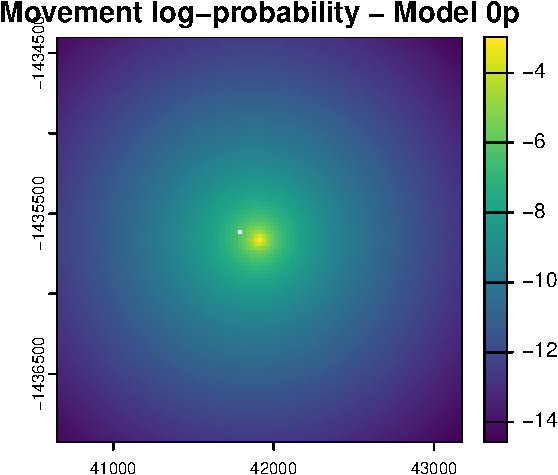
\includegraphics[keepaspectratio]{ssf_validation_files/figure-pdf/unnamed-chunk-8-2.pdf}}

\begin{verbatim}
        x_       y_                   t_   id      x1_      y1_     x2_
3 41779.44 -1435601 2018-07-25T03:04:17Z 2005 41779.44 -1435601 41841.2
       y2_  x2_cent   y2_cent                  t2_ t_diff hour_t1 yday_t1
3 -1435635 61.76368 -34.32294 2018-07-25T04:04:39Z      1      13     206
  hour_t2 hour_t2_sin hour_t2_cos yday_t2 yday_t2_sin yday_t2_cos       sl
3      14        -0.5  -0.8660254     206  -0.3913578  -0.9202386 70.65986
    log_sl    bearing bearing_sin bearing_cos       ta     cos_ta    x_min
3 4.257878 -0.5072195  -0.4857487   0.8740985 2.994917 -0.9892624 40516.94
     x_max    y_min    y_max s2_index points_vect_cent year_t2
3 43041.94 -1436863 -1434338        7               NA    2018
  yday_t2_2018_base prob_habitat_ssf_0p prob_movement_ssf_0p
3               206                  NA                   NA
  prob_next_step_ssf_0p
3                    NA
\end{verbatim}

\pandocbounded{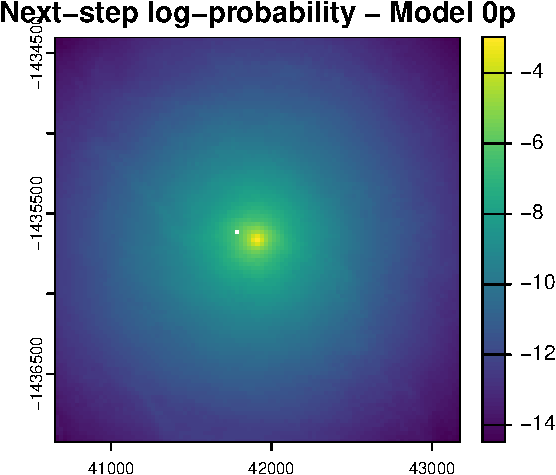
\includegraphics[keepaspectratio]{ssf_validation_files/figure-pdf/unnamed-chunk-8-3.pdf}}

\pandocbounded{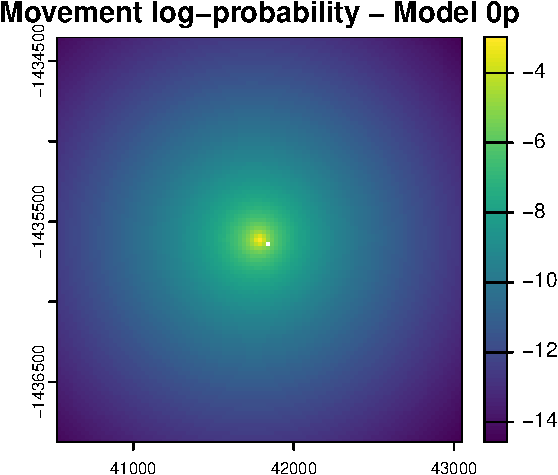
\includegraphics[keepaspectratio]{ssf_validation_files/figure-pdf/unnamed-chunk-8-4.pdf}}

\begin{verbatim}
       x_       y_                   t_   id     x1_      y1_      x2_      y2_
4 41841.2 -1435635 2018-07-25T04:04:39Z 2005 41841.2 -1435635 41655.46 -1435604
    x2_cent  y2_cent                  t2_ t_diff hour_t1 yday_t1 hour_t2
4 -185.7399 31.00353 2018-07-25T05:04:27Z      1      14     206      15
  hour_t2_sin hour_t2_cos yday_t2 yday_t2_sin yday_t2_cos       sl   log_sl
4  -0.7071068  -0.7071068     206  -0.3913578  -0.9202386 188.3097 5.238088
   bearing bearing_sin bearing_cos        ta     cos_ta   x_min   x_max
4 2.976198   0.1646412  -0.9863535 -2.799767 -0.9421444 40578.7 43103.7
     y_min    y_max s2_index points_vect_cent year_t2 yday_t2_2018_base
4 -1436898 -1434373        7               NA    2018               206
  prob_habitat_ssf_0p prob_movement_ssf_0p prob_next_step_ssf_0p
4                  NA                   NA                    NA
\end{verbatim}

\pandocbounded{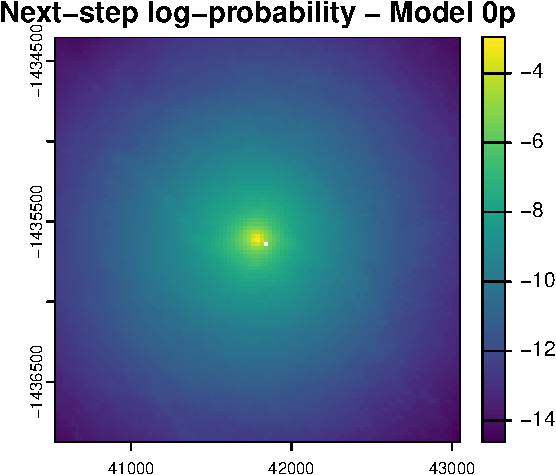
\includegraphics[keepaspectratio]{ssf_validation_files/figure-pdf/unnamed-chunk-8-5.pdf}}

\pandocbounded{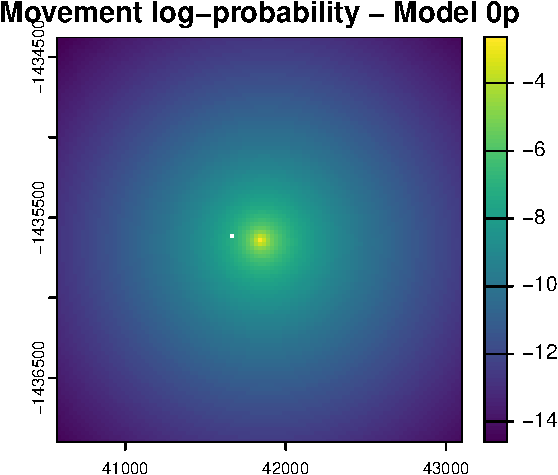
\includegraphics[keepaspectratio]{ssf_validation_files/figure-pdf/unnamed-chunk-8-6.pdf}}

\begin{verbatim}
        x_       y_                   t_   id      x1_      y1_      x2_
5 41655.46 -1435604 2018-07-25T05:04:27Z 2005 41655.46 -1435604 41618.65
       y2_   x2_cent   y2_cent                  t2_ t_diff hour_t1 yday_t1
5 -1435608 -36.81141 -4.438037 2018-07-25T06:04:24Z      1      15     206
  hour_t2 hour_t2_sin hour_t2_cos yday_t2 yday_t2_sin yday_t2_cos       sl
5      16  -0.8660254        -0.5     206  -0.3913578  -0.9202386 37.07797
    log_sl  bearing bearing_sin bearing_cos        ta    cos_ta    x_min
5 3.613023 -3.02161  -0.1196947  -0.9928107 0.2853766 0.9595557 40392.96
     x_max    y_min    y_max s2_index points_vect_cent year_t2
5 42917.96 -1436867 -1434342        7               NA    2018
  yday_t2_2018_base prob_habitat_ssf_0p prob_movement_ssf_0p
5               206                  NA                   NA
  prob_next_step_ssf_0p
5                    NA
\end{verbatim}

\pandocbounded{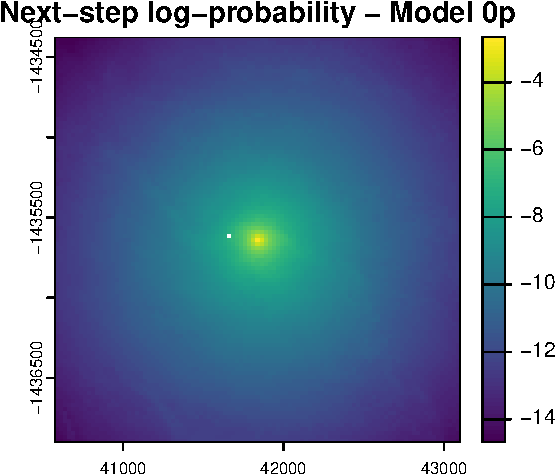
\includegraphics[keepaspectratio]{ssf_validation_files/figure-pdf/unnamed-chunk-8-7.pdf}}

\pandocbounded{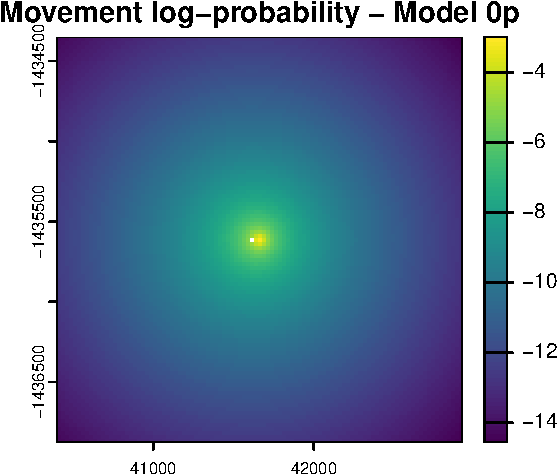
\includegraphics[keepaspectratio]{ssf_validation_files/figure-pdf/unnamed-chunk-8-8.pdf}}

\begin{verbatim}
        x_       y_                   t_   id      x1_      y1_      x2_
6 41618.65 -1435608 2018-07-25T06:04:24Z 2005 41618.65 -1435608 41688.44
       y2_  x2_cent   y2_cent                  t2_ t_diff hour_t1 yday_t1
6 -1436126 69.78648 -517.1566 2018-07-25T07:04:28Z      1      16     206
  hour_t2 hour_t2_sin hour_t2_cos yday_t2 yday_t2_sin yday_t2_cos       sl
6      17  -0.9659258   -0.258819     206  -0.3913578  -0.9202386 521.8439
    log_sl   bearing bearing_sin bearing_cos       ta      cos_ta    x_min
6 6.257369 -1.436664  -0.9910177   0.1337306 1.584946 -0.01414957 40356.15
     x_max    y_min    y_max s2_index points_vect_cent year_t2
6 42881.15 -1436871 -1434346        7               NA    2018
  yday_t2_2018_base prob_habitat_ssf_0p prob_movement_ssf_0p
6               206                  NA                   NA
  prob_next_step_ssf_0p
6                    NA
\end{verbatim}

\pandocbounded{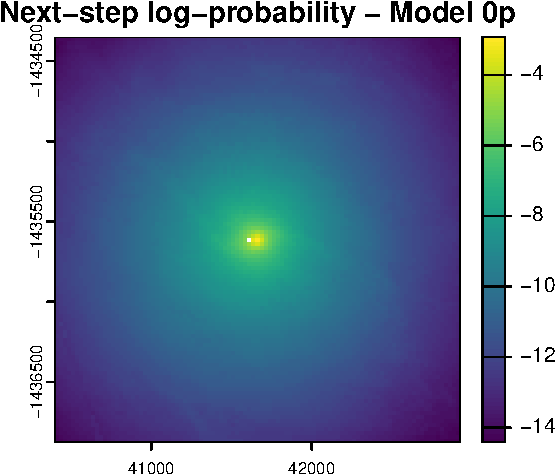
\includegraphics[keepaspectratio]{ssf_validation_files/figure-pdf/unnamed-chunk-8-9.pdf}}

\pandocbounded{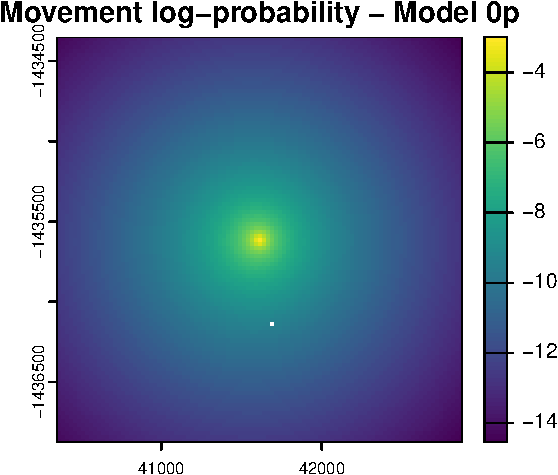
\includegraphics[keepaspectratio]{ssf_validation_files/figure-pdf/unnamed-chunk-8-10.pdf}}

\begin{verbatim}
        x_       y_                   t_   id      x1_      y1_      x2_
7 41688.44 -1436126 2018-07-25T07:04:28Z 2005 41688.44 -1436126 41684.34
       y2_   x2_cent  y2_cent                  t2_ t_diff hour_t1 yday_t1
7 -1436119 -4.095906 7.020228 2018-07-25T08:04:31Z      1      17     206
  hour_t2 hour_t2_sin  hour_t2_cos yday_t2 yday_t2_sin yday_t2_cos       sl
7      18          -1 -1.83691e-16     206  -0.3913578  -0.9202386 8.127733
    log_sl  bearing bearing_sin bearing_cos        ta     cos_ta    x_min
7 2.095282 2.098953   0.8637375   -0.503942 -2.747568 -0.9233716 40425.94
     x_max    y_min    y_max s2_index points_vect_cent year_t2
7 42950.94 -1437388 -1434863        7               NA    2018
  yday_t2_2018_base prob_habitat_ssf_0p prob_movement_ssf_0p
7               206                  NA                   NA
  prob_next_step_ssf_0p
7                    NA
\end{verbatim}

\pandocbounded{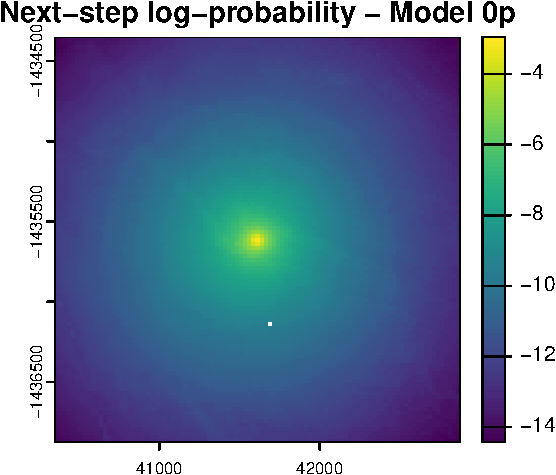
\includegraphics[keepaspectratio]{ssf_validation_files/figure-pdf/unnamed-chunk-8-11.pdf}}

\pandocbounded{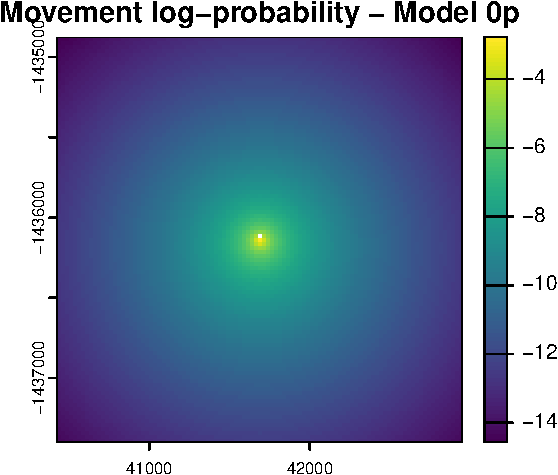
\includegraphics[keepaspectratio]{ssf_validation_files/figure-pdf/unnamed-chunk-8-12.pdf}}

\begin{verbatim}
        x_       y_                   t_   id      x1_      y1_      x2_
8 41684.34 -1436119 2018-07-25T08:04:31Z 2005 41684.34 -1436119 41674.59
       y2_   x2_cent     y2_cent                  t2_ t_diff hour_t1 yday_t1
8 -1436119 -9.754289 -0.08369654 2018-07-25T09:04:33Z      1      18     206
  hour_t2 hour_t2_sin hour_t2_cos yday_t2 yday_t2_sin yday_t2_cos       sl
8      19  -0.9659258    0.258819     206  -0.3913578  -0.9202386 9.754648
    log_sl   bearing bearing_sin bearing_cos      ta    cos_ta    x_min
8 2.277744 -3.133012 -0.00858017  -0.9999632 1.05122 0.4965124 40421.84
     x_max    y_min    y_max s2_index points_vect_cent year_t2
8 42946.84 -1437381 -1434856        7               NA    2018
  yday_t2_2018_base prob_habitat_ssf_0p prob_movement_ssf_0p
8               206                  NA                   NA
  prob_next_step_ssf_0p
8                    NA
\end{verbatim}

\pandocbounded{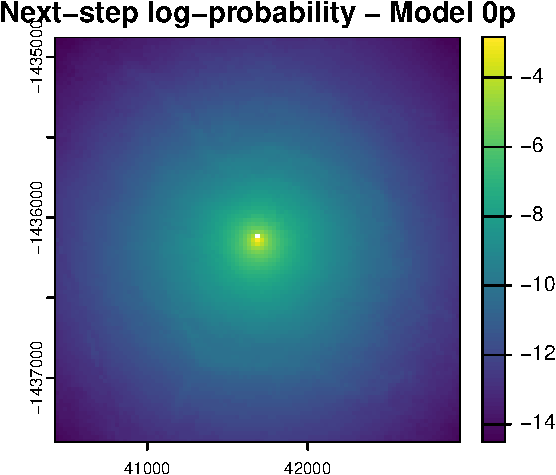
\includegraphics[keepaspectratio]{ssf_validation_files/figure-pdf/unnamed-chunk-8-13.pdf}}

\pandocbounded{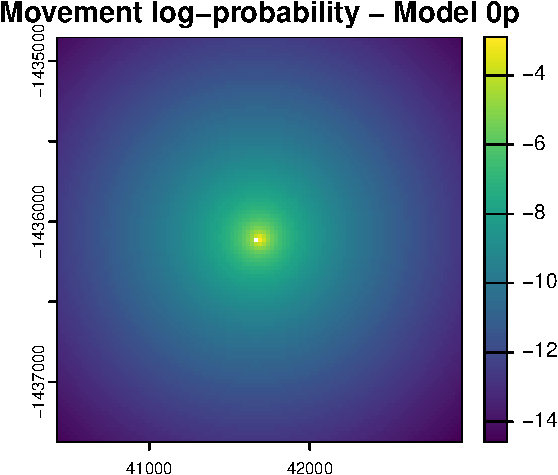
\includegraphics[keepaspectratio]{ssf_validation_files/figure-pdf/unnamed-chunk-8-14.pdf}}

\begin{verbatim}
        x_       y_                   t_   id      x1_      y1_      x2_
9 41674.59 -1436119 2018-07-25T09:04:33Z 2005 41674.59 -1436119 41425.16
       y2_   x2_cent  y2_cent                  t2_ t_diff hour_t1 yday_t1
9 -1435938 -249.4296 180.3333 2018-07-25T10:04:02Z      1      19     206
  hour_t2 hour_t2_sin hour_t2_cos yday_t2 yday_t2_sin yday_t2_cos       sl
9      20  -0.8660254         0.5     206  -0.3913578  -0.9202386 307.7908
   log_sl  bearing bearing_sin bearing_cos         ta    cos_ta    x_min
9 5.72942 2.515608   0.5858955  -0.8103866 -0.6345649 0.8053297 40412.09
     x_max    y_min    y_max s2_index points_vect_cent year_t2
9 42937.09 -1437381 -1434856        7               NA    2018
  yday_t2_2018_base prob_habitat_ssf_0p prob_movement_ssf_0p
9               206                  NA                   NA
  prob_next_step_ssf_0p
9                    NA
\end{verbatim}

\pandocbounded{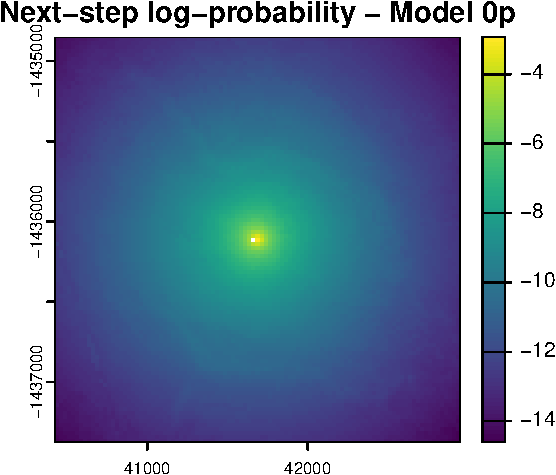
\includegraphics[keepaspectratio]{ssf_validation_files/figure-pdf/unnamed-chunk-8-15.pdf}}

\pandocbounded{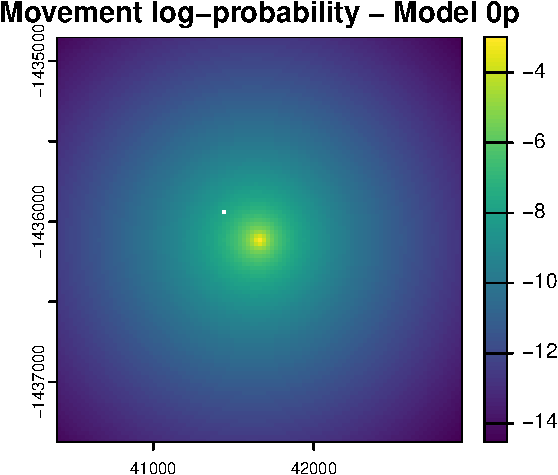
\includegraphics[keepaspectratio]{ssf_validation_files/figure-pdf/unnamed-chunk-8-16.pdf}}

\begin{verbatim}
         x_       y_                   t_   id      x1_      y1_      x2_
10 41425.16 -1435938 2018-07-25T10:04:02Z 2005 41425.16 -1435938 40563.21
        y2_   x2_cent  y2_cent                  t2_ t_diff hour_t1 yday_t1
10 -1435841 -861.9445 97.45269 2018-07-25T11:04:04Z      1      20     206
   hour_t2 hour_t2_sin hour_t2_cos yday_t2 yday_t2_sin yday_t2_cos       sl
10      21  -0.7071068   0.7071068     206  -0.3913578  -0.9202386 867.4361
     log_sl  bearing bearing_sin bearing_cos        ta    cos_ta    x_min
10 6.765542 3.029009   0.1123457  -0.9936692 0.5134012 0.8710791 40162.66
      x_max    y_min    y_max s2_index points_vect_cent year_t2
10 42687.66 -1437201 -1434676        7               NA    2018
   yday_t2_2018_base prob_habitat_ssf_0p prob_movement_ssf_0p
10               206                  NA                   NA
   prob_next_step_ssf_0p
10                    NA
\end{verbatim}

\pandocbounded{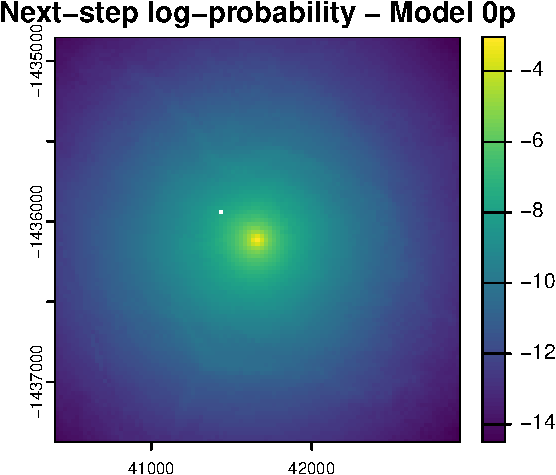
\includegraphics[keepaspectratio]{ssf_validation_files/figure-pdf/unnamed-chunk-8-17.pdf}}

\pandocbounded{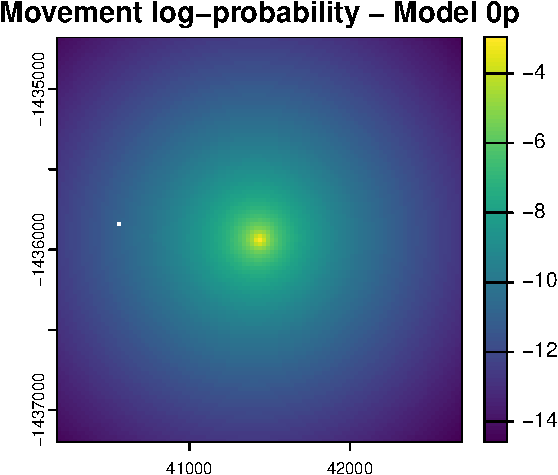
\includegraphics[keepaspectratio]{ssf_validation_files/figure-pdf/unnamed-chunk-8-18.pdf}}

\begin{verbatim}
         x_       y_                   t_   id      x1_      y1_      x2_
11 40563.21 -1435841 2018-07-25T11:04:04Z 2005 40563.21 -1435841 40512.76
        y2_   x2_cent  y2_cent                  t2_ t_diff hour_t1 yday_t1
11 -1435777 -50.44988 63.87376 2018-07-25T12:05:13Z      1      21     206
   hour_t2 hour_t2_sin hour_t2_cos yday_t2 yday_t2_sin yday_t2_cos       sl
11      22        -0.5   0.8660254     206  -0.3913578  -0.9202386 81.39439
     log_sl bearing bearing_sin bearing_cos         ta    cos_ta    x_min
11 4.399306 2.23931    0.784744    -0.61982 -0.7896996 0.7040587 39300.71
      x_max    y_min    y_max s2_index points_vect_cent year_t2
11 41825.71 -1437103 -1434578        7               NA    2018
   yday_t2_2018_base prob_habitat_ssf_0p prob_movement_ssf_0p
11               206                  NA                   NA
   prob_next_step_ssf_0p
11                    NA
\end{verbatim}

\pandocbounded{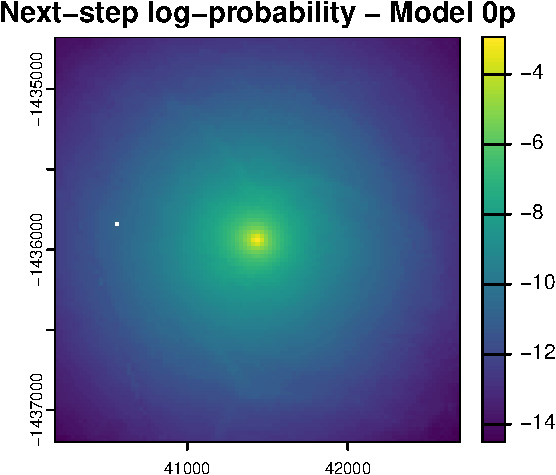
\includegraphics[keepaspectratio]{ssf_validation_files/figure-pdf/unnamed-chunk-8-19.pdf}}

\pandocbounded{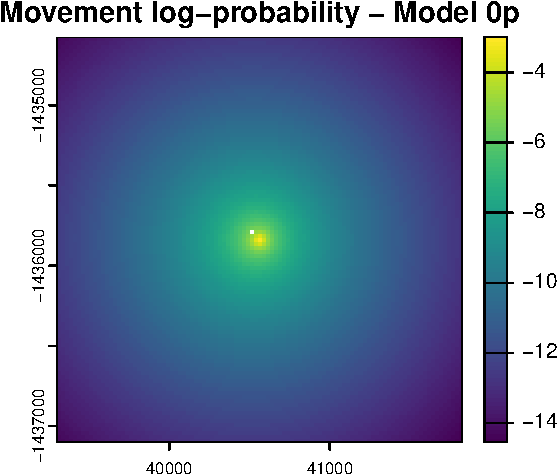
\includegraphics[keepaspectratio]{ssf_validation_files/figure-pdf/unnamed-chunk-8-20.pdf}}

\pandocbounded{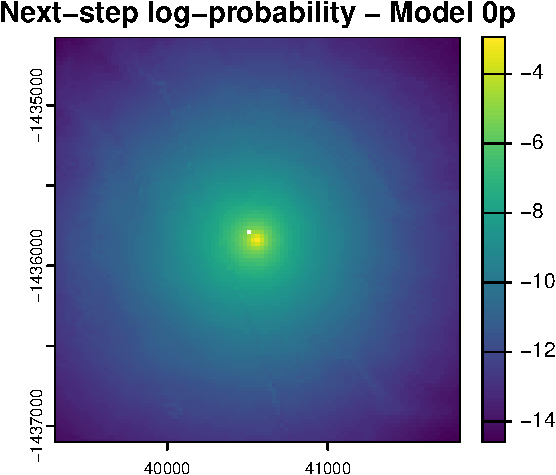
\includegraphics[keepaspectratio]{ssf_validation_files/figure-pdf/unnamed-chunk-8-21.pdf}}

\begin{verbatim}
33.56 sec elapsed
[1] "ssf_coefficients/id2005_2pDaily_coefs_80-10-10_2025-04-10.csv"
\end{verbatim}

\begin{verbatim}
Rows: 240 Columns: 13
-- Column specification --------------------------------------------------------
Delimiter: ","
dbl (13): hour, ndvi, ndvi_2, canopy, canopy_2, slope, herby, sl, log_sl, co...

i Use `spec()` to retrieve the full column specification for this data.
i Specify the column types or set `show_col_types = FALSE` to quiet this message.
\end{verbatim}

\begin{verbatim}
Warning in max(values(move_log), na.rm = T): no non-missing arguments to max;
returning -Inf
\end{verbatim}

\begin{verbatim}
Warning in max(values(move_log), na.rm = T): no non-missing arguments to max;
returning -Inf
\end{verbatim}

\begin{verbatim}
Warning in max(values(next_step_log), na.rm = T): no non-missing arguments to
max; returning -Inf
Warning in max(values(next_step_log), na.rm = T): no non-missing arguments to
max; returning -Inf
\end{verbatim}

\begin{verbatim}
Warning: Failed to compute min/max, no valid pixels found in sampling. (GDAL
error 1)
\end{verbatim}

\begin{verbatim}
        x_       y_                   t_   id      x1_      y1_      x2_
1 41969.31 -1435671 2018-07-25T01:04:23Z 2005 41969.31 -1435671 41921.52
       y2_   x2_cent  y2_cent                  t2_ t_diff hour_t1 yday_t1
1 -1435654 -47.78894 16.85711 2018-07-25T02:04:39Z      1      11     206
  hour_t2  hour_t2_sin hour_t2_cos yday_t2 yday_t2_sin yday_t2_cos       sl
1      12 1.224606e-16          -1     206  -0.3913578  -0.9202386 50.67489
    log_sl  bearing bearing_sin bearing_cos       ta   cos_ta    x_min    x_max
1 3.925431 2.802478   0.3326521  -0.9430496 1.367942 0.201466 40706.81 43231.81
     y_min    y_max s2_index points_vect_cent year_t2 yday_t2_2018_base
1 -1436934 -1434409        7               NA    2018               206
  prob_habitat_ssf_0p prob_movement_ssf_0p prob_next_step_ssf_0p
1        9.615473e-05                   NA                    NA
\end{verbatim}

\begin{verbatim}
Warning: Failed to compute min/max, no valid pixels found in sampling. (GDAL
error 1)
\end{verbatim}

\pandocbounded{
\includegraphics[keepaspectratio]{ssf_validation_files/figure-pdf/unnamed-chunk-8-22.pdf}}

\begin{verbatim}
Warning: Failed to compute min/max, no valid pixels found in sampling. (GDAL
error 1)
\end{verbatim}

\begin{verbatim}
        x_       y_                   t_   id      x1_      y1_      x2_
2 41921.52 -1435654 2018-07-25T02:04:39Z 2005 41921.52 -1435654 41779.44
       y2_   x2_cent  y2_cent                  t2_ t_diff hour_t1 yday_t1
2 -1435601 -142.0823 53.56843 2018-07-25T03:04:17Z      1      12     206
  hour_t2 hour_t2_sin hour_t2_cos yday_t2 yday_t2_sin yday_t2_cos       sl
2      13   -0.258819  -0.9659258     206  -0.3913578  -0.9202386 151.8452
    log_sl  bearing bearing_sin bearing_cos          ta    cos_ta    x_min
2 5.022862 2.781049   0.3527831  -0.9357051 -0.02142933 0.9997704 40659.02
     x_max    y_min    y_max s2_index points_vect_cent year_t2
2 43184.02 -1436917 -1434392        7               NA    2018
  yday_t2_2018_base prob_habitat_ssf_0p prob_movement_ssf_0p
2               206         9.65375e-05          0.001913733
  prob_next_step_ssf_0p prob_habitat_ssf_2p prob_movement_ssf_2p
2           0.001924442                  NA                   NA
  prob_next_step_ssf_2p
2                    NA
\end{verbatim}

\pandocbounded{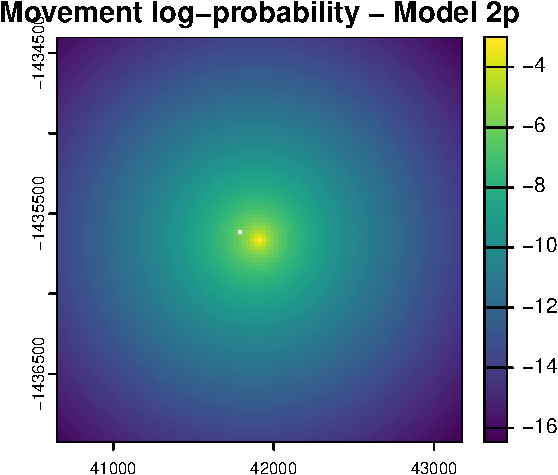
\includegraphics[keepaspectratio]{ssf_validation_files/figure-pdf/unnamed-chunk-8-23.pdf}}

\begin{verbatim}
        x_       y_                   t_   id      x1_      y1_     x2_
3 41779.44 -1435601 2018-07-25T03:04:17Z 2005 41779.44 -1435601 41841.2
       y2_  x2_cent   y2_cent                  t2_ t_diff hour_t1 yday_t1
3 -1435635 61.76368 -34.32294 2018-07-25T04:04:39Z      1      13     206
  hour_t2 hour_t2_sin hour_t2_cos yday_t2 yday_t2_sin yday_t2_cos       sl
3      14        -0.5  -0.8660254     206  -0.3913578  -0.9202386 70.65986
    log_sl    bearing bearing_sin bearing_cos       ta     cos_ta    x_min
3 4.257878 -0.5072195  -0.4857487   0.8740985 2.994917 -0.9892624 40516.94
     x_max    y_min    y_max s2_index points_vect_cent year_t2
3 43041.94 -1436863 -1434338        7               NA    2018
  yday_t2_2018_base prob_habitat_ssf_0p prob_movement_ssf_0p
3               206        9.361172e-05          0.005811244
  prob_next_step_ssf_0p prob_habitat_ssf_2p prob_movement_ssf_2p
3           0.005718225                  NA                   NA
  prob_next_step_ssf_2p
3                    NA
\end{verbatim}

\pandocbounded{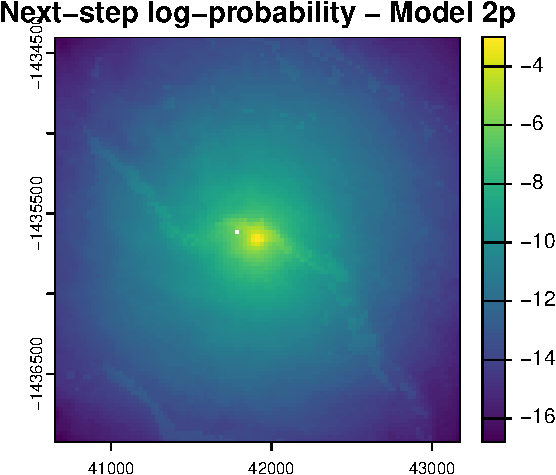
\includegraphics[keepaspectratio]{ssf_validation_files/figure-pdf/unnamed-chunk-8-24.pdf}}

\pandocbounded{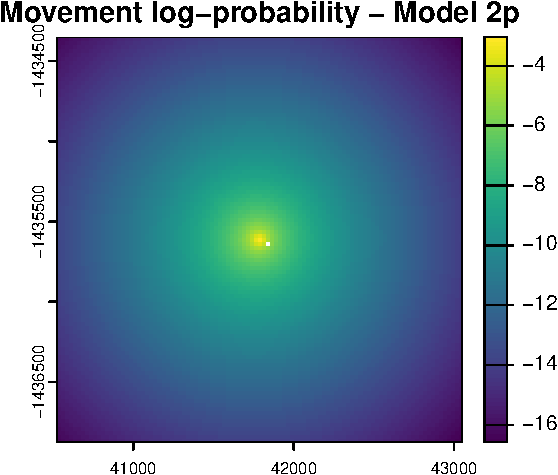
\includegraphics[keepaspectratio]{ssf_validation_files/figure-pdf/unnamed-chunk-8-25.pdf}}

\begin{verbatim}
       x_       y_                   t_   id     x1_      y1_      x2_      y2_
4 41841.2 -1435635 2018-07-25T04:04:39Z 2005 41841.2 -1435635 41655.46 -1435604
    x2_cent  y2_cent                  t2_ t_diff hour_t1 yday_t1 hour_t2
4 -185.7399 31.00353 2018-07-25T05:04:27Z      1      14     206      15
  hour_t2_sin hour_t2_cos yday_t2 yday_t2_sin yday_t2_cos       sl   log_sl
4  -0.7071068  -0.7071068     206  -0.3913578  -0.9202386 188.3097 5.238088
   bearing bearing_sin bearing_cos        ta     cos_ta   x_min   x_max
4 2.976198   0.1646412  -0.9863535 -2.799767 -0.9421444 40578.7 43103.7
     y_min    y_max s2_index points_vect_cent year_t2 yday_t2_2018_base
4 -1436898 -1434373        7               NA    2018               206
  prob_habitat_ssf_0p prob_movement_ssf_0p prob_next_step_ssf_0p
4        9.907641e-05         0.0007681248           0.000797917
  prob_habitat_ssf_2p prob_movement_ssf_2p prob_next_step_ssf_2p
4                  NA                   NA                    NA
\end{verbatim}

\pandocbounded{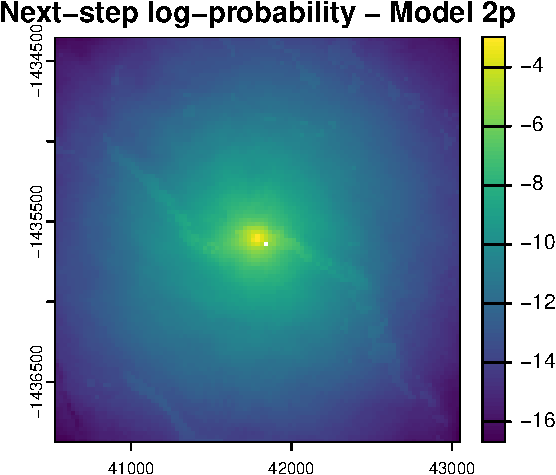
\includegraphics[keepaspectratio]{ssf_validation_files/figure-pdf/unnamed-chunk-8-26.pdf}}

\pandocbounded{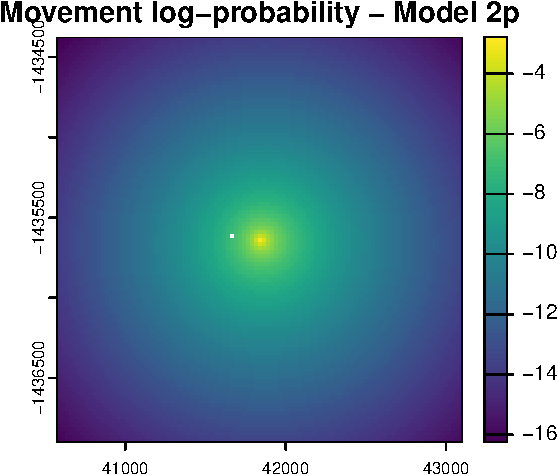
\includegraphics[keepaspectratio]{ssf_validation_files/figure-pdf/unnamed-chunk-8-27.pdf}}

\begin{verbatim}
        x_       y_                   t_   id      x1_      y1_      x2_
5 41655.46 -1435604 2018-07-25T05:04:27Z 2005 41655.46 -1435604 41618.65
       y2_   x2_cent   y2_cent                  t2_ t_diff hour_t1 yday_t1
5 -1435608 -36.81141 -4.438037 2018-07-25T06:04:24Z      1      15     206
  hour_t2 hour_t2_sin hour_t2_cos yday_t2 yday_t2_sin yday_t2_cos       sl
5      16  -0.8660254        -0.5     206  -0.3913578  -0.9202386 37.07797
    log_sl  bearing bearing_sin bearing_cos        ta    cos_ta    x_min
5 3.613023 -3.02161  -0.1196947  -0.9928107 0.2853766 0.9595557 40392.96
     x_max    y_min    y_max s2_index points_vect_cent year_t2
5 42917.96 -1436867 -1434342        7               NA    2018
  yday_t2_2018_base prob_habitat_ssf_0p prob_movement_ssf_0p
5               206        9.602568e-05           0.01028661
  prob_next_step_ssf_0p prob_habitat_ssf_2p prob_movement_ssf_2p
5            0.01055869                  NA                   NA
  prob_next_step_ssf_2p
5                    NA
\end{verbatim}

\pandocbounded{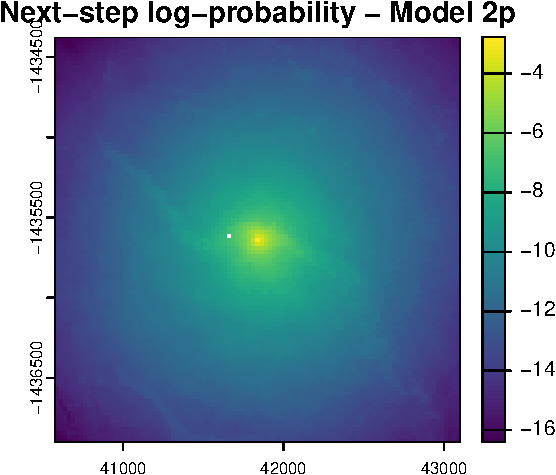
\includegraphics[keepaspectratio]{ssf_validation_files/figure-pdf/unnamed-chunk-8-28.pdf}}

\pandocbounded{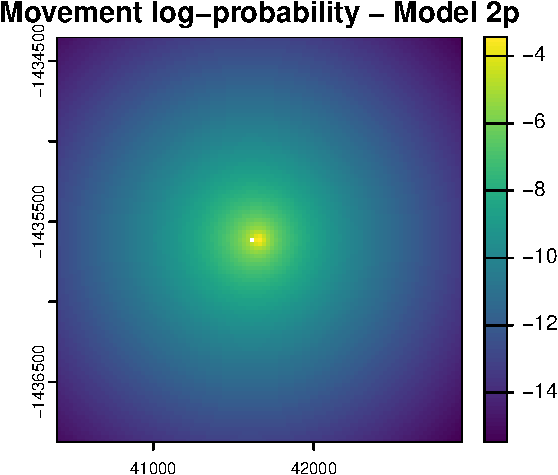
\includegraphics[keepaspectratio]{ssf_validation_files/figure-pdf/unnamed-chunk-8-29.pdf}}

\begin{verbatim}
        x_       y_                   t_   id      x1_      y1_      x2_
6 41618.65 -1435608 2018-07-25T06:04:24Z 2005 41618.65 -1435608 41688.44
       y2_  x2_cent   y2_cent                  t2_ t_diff hour_t1 yday_t1
6 -1436126 69.78648 -517.1566 2018-07-25T07:04:28Z      1      16     206
  hour_t2 hour_t2_sin hour_t2_cos yday_t2 yday_t2_sin yday_t2_cos       sl
6      17  -0.9659258   -0.258819     206  -0.3913578  -0.9202386 521.8439
    log_sl   bearing bearing_sin bearing_cos       ta      cos_ta    x_min
6 6.257369 -1.436664  -0.9910177   0.1337306 1.584946 -0.01414957 40356.15
     x_max    y_min    y_max s2_index points_vect_cent year_t2
6 42881.15 -1436871 -1434346        7               NA    2018
  yday_t2_2018_base prob_habitat_ssf_0p prob_movement_ssf_0p
6               206        9.083069e-05         7.547135e-05
  prob_next_step_ssf_0p prob_habitat_ssf_2p prob_movement_ssf_2p
6          7.375487e-05                  NA                   NA
  prob_next_step_ssf_2p
6                    NA
\end{verbatim}

\pandocbounded{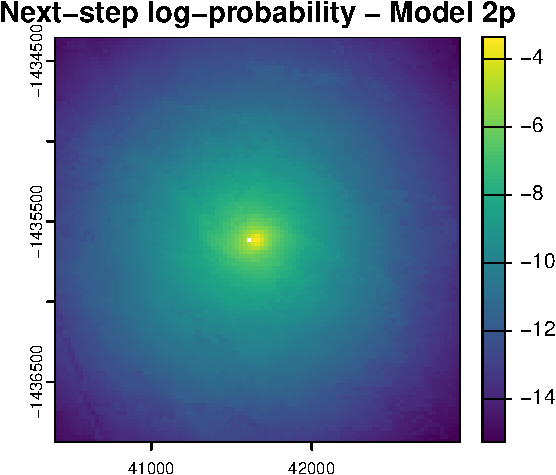
\includegraphics[keepaspectratio]{ssf_validation_files/figure-pdf/unnamed-chunk-8-30.pdf}}

\pandocbounded{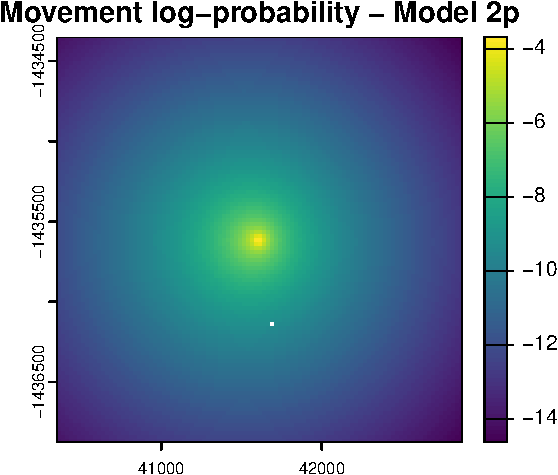
\includegraphics[keepaspectratio]{ssf_validation_files/figure-pdf/unnamed-chunk-8-31.pdf}}

\begin{verbatim}
        x_       y_                   t_   id      x1_      y1_      x2_
7 41688.44 -1436126 2018-07-25T07:04:28Z 2005 41688.44 -1436126 41684.34
       y2_   x2_cent  y2_cent                  t2_ t_diff hour_t1 yday_t1
7 -1436119 -4.095906 7.020228 2018-07-25T08:04:31Z      1      17     206
  hour_t2 hour_t2_sin  hour_t2_cos yday_t2 yday_t2_sin yday_t2_cos       sl
7      18          -1 -1.83691e-16     206  -0.3913578  -0.9202386 8.127733
    log_sl  bearing bearing_sin bearing_cos        ta     cos_ta    x_min
7 2.095282 2.098953   0.8637375   -0.503942 -2.747568 -0.9233716 40425.94
     x_max    y_min    y_max s2_index points_vect_cent year_t2
7 42950.94 -1437388 -1434863        7               NA    2018
  yday_t2_2018_base prob_habitat_ssf_0p prob_movement_ssf_0p
7               206        9.167352e-05           0.02051778
  prob_next_step_ssf_0p prob_habitat_ssf_2p prob_movement_ssf_2p
7            0.01968547                  NA                   NA
  prob_next_step_ssf_2p
7                    NA
\end{verbatim}

\pandocbounded{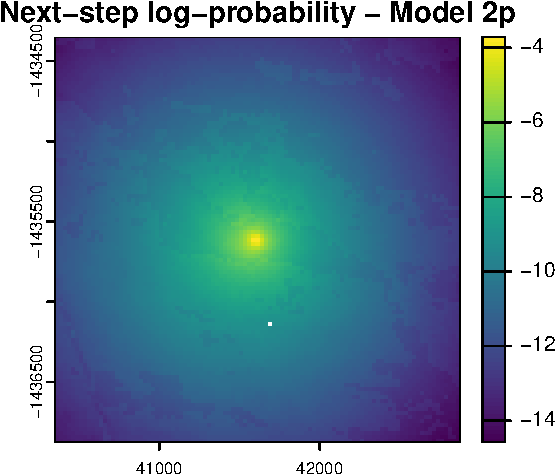
\includegraphics[keepaspectratio]{ssf_validation_files/figure-pdf/unnamed-chunk-8-32.pdf}}

\pandocbounded{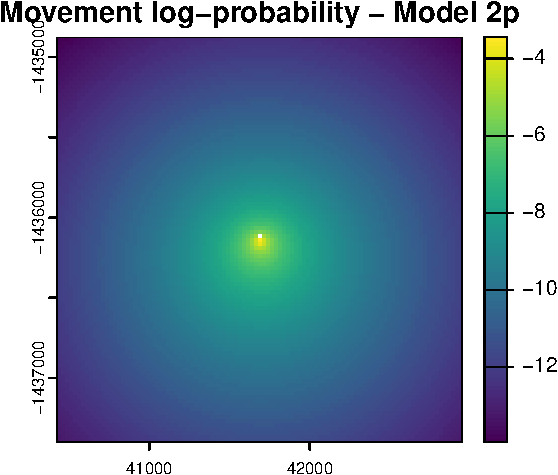
\includegraphics[keepaspectratio]{ssf_validation_files/figure-pdf/unnamed-chunk-8-33.pdf}}

\begin{verbatim}
        x_       y_                   t_   id      x1_      y1_      x2_
8 41684.34 -1436119 2018-07-25T08:04:31Z 2005 41684.34 -1436119 41674.59
       y2_   x2_cent     y2_cent                  t2_ t_diff hour_t1 yday_t1
8 -1436119 -9.754289 -0.08369654 2018-07-25T09:04:33Z      1      18     206
  hour_t2 hour_t2_sin hour_t2_cos yday_t2 yday_t2_sin yday_t2_cos       sl
8      19  -0.9659258    0.258819     206  -0.3913578  -0.9202386 9.754648
    log_sl   bearing bearing_sin bearing_cos      ta    cos_ta    x_min
8 2.277744 -3.133012 -0.00858017  -0.9999632 1.05122 0.4965124 40421.84
     x_max    y_min    y_max s2_index points_vect_cent year_t2
8 42946.84 -1437381 -1434856        7               NA    2018
  yday_t2_2018_base prob_habitat_ssf_0p prob_movement_ssf_0p
8               206        9.007231e-05           0.02774303
  prob_next_step_ssf_0p prob_habitat_ssf_2p prob_movement_ssf_2p
8            0.02635727                  NA                   NA
  prob_next_step_ssf_2p
8                    NA
\end{verbatim}

\pandocbounded{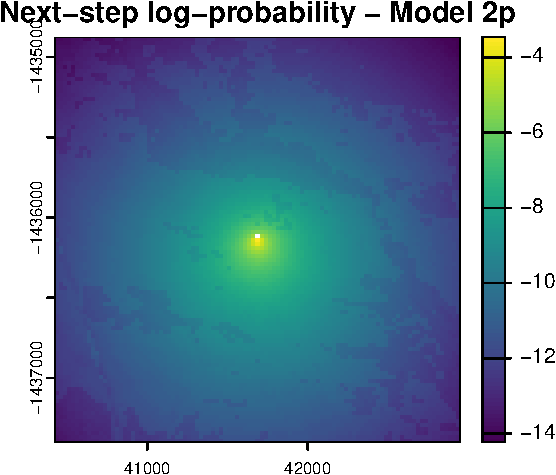
\includegraphics[keepaspectratio]{ssf_validation_files/figure-pdf/unnamed-chunk-8-34.pdf}}

\pandocbounded{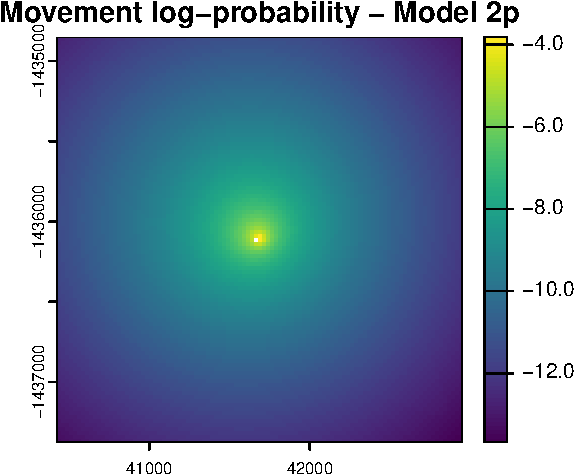
\includegraphics[keepaspectratio]{ssf_validation_files/figure-pdf/unnamed-chunk-8-35.pdf}}

\begin{verbatim}
        x_       y_                   t_   id      x1_      y1_      x2_
9 41674.59 -1436119 2018-07-25T09:04:33Z 2005 41674.59 -1436119 41425.16
       y2_   x2_cent  y2_cent                  t2_ t_diff hour_t1 yday_t1
9 -1435938 -249.4296 180.3333 2018-07-25T10:04:02Z      1      19     206
  hour_t2 hour_t2_sin hour_t2_cos yday_t2 yday_t2_sin yday_t2_cos       sl
9      20  -0.8660254         0.5     206  -0.3913578  -0.9202386 307.7908
   log_sl  bearing bearing_sin bearing_cos         ta    cos_ta    x_min
9 5.72942 2.515608   0.5858955  -0.8103866 -0.6345649 0.8053297 40412.09
     x_max    y_min    y_max s2_index points_vect_cent year_t2
9 42937.09 -1437381 -1434856        7               NA    2018
  yday_t2_2018_base prob_habitat_ssf_0p prob_movement_ssf_0p
9               206        9.566552e-05         0.0004125345
  prob_next_step_ssf_0p prob_habitat_ssf_2p prob_movement_ssf_2p
9          0.0004177971                  NA                   NA
  prob_next_step_ssf_2p
9                    NA
\end{verbatim}

\pandocbounded{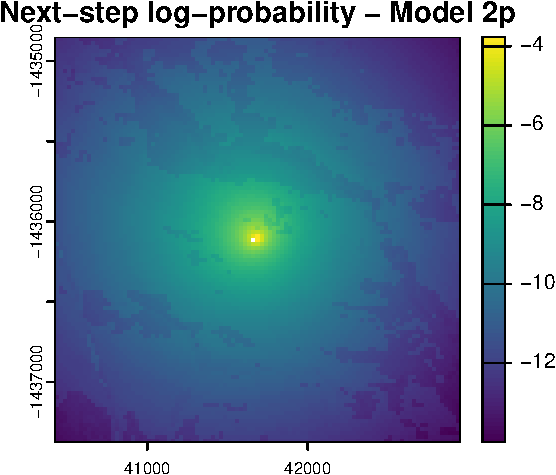
\includegraphics[keepaspectratio]{ssf_validation_files/figure-pdf/unnamed-chunk-8-36.pdf}}

\pandocbounded{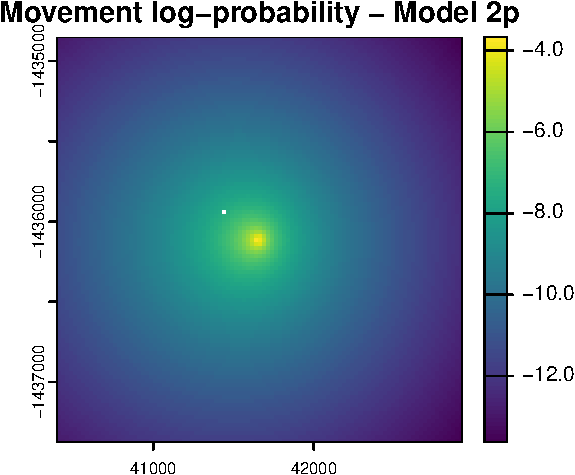
\includegraphics[keepaspectratio]{ssf_validation_files/figure-pdf/unnamed-chunk-8-37.pdf}}

\begin{verbatim}
         x_       y_                   t_   id      x1_      y1_      x2_
10 41425.16 -1435938 2018-07-25T10:04:02Z 2005 41425.16 -1435938 40563.21
        y2_   x2_cent  y2_cent                  t2_ t_diff hour_t1 yday_t1
10 -1435841 -861.9445 97.45269 2018-07-25T11:04:04Z      1      20     206
   hour_t2 hour_t2_sin hour_t2_cos yday_t2 yday_t2_sin yday_t2_cos       sl
10      21  -0.7071068   0.7071068     206  -0.3913578  -0.9202386 867.4361
     log_sl  bearing bearing_sin bearing_cos        ta    cos_ta    x_min
10 6.765542 3.029009   0.1123457  -0.9936692 0.5134012 0.8710791 40162.66
      x_max    y_min    y_max s2_index points_vect_cent year_t2
10 42687.66 -1437201 -1434676        7               NA    2018
   yday_t2_2018_base prob_habitat_ssf_0p prob_movement_ssf_0p
10               206         0.000109441          1.74964e-05
   prob_next_step_ssf_0p prob_habitat_ssf_2p prob_movement_ssf_2p
10          2.029205e-05                  NA                   NA
   prob_next_step_ssf_2p
10                    NA
\end{verbatim}

\pandocbounded{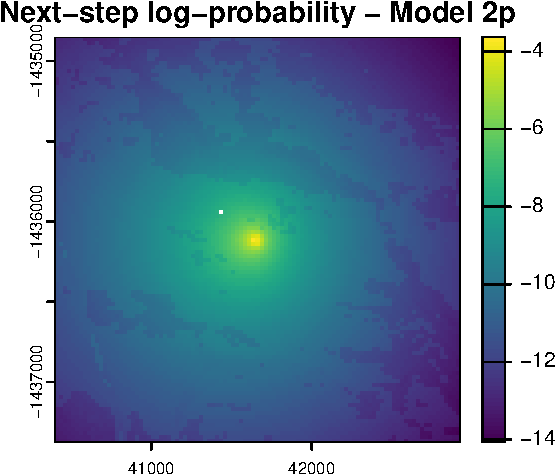
\includegraphics[keepaspectratio]{ssf_validation_files/figure-pdf/unnamed-chunk-8-38.pdf}}

\pandocbounded{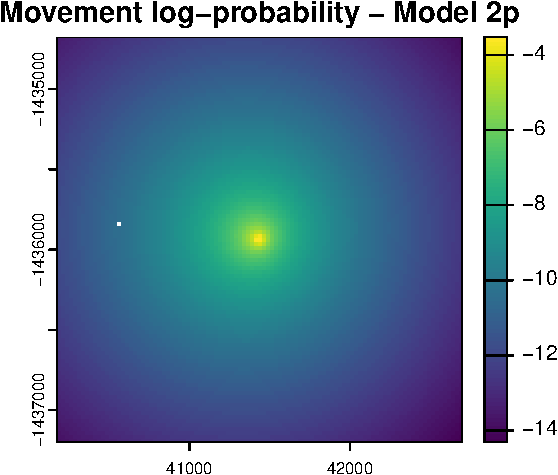
\includegraphics[keepaspectratio]{ssf_validation_files/figure-pdf/unnamed-chunk-8-39.pdf}}

\begin{verbatim}
         x_       y_                   t_   id      x1_      y1_      x2_
11 40563.21 -1435841 2018-07-25T11:04:04Z 2005 40563.21 -1435841 40512.76
        y2_   x2_cent  y2_cent                  t2_ t_diff hour_t1 yday_t1
11 -1435777 -50.44988 63.87376 2018-07-25T12:05:13Z      1      21     206
   hour_t2 hour_t2_sin hour_t2_cos yday_t2 yday_t2_sin yday_t2_cos       sl
11      22        -0.5   0.8660254     206  -0.3913578  -0.9202386 81.39439
     log_sl bearing bearing_sin bearing_cos         ta    cos_ta    x_min
11 4.399306 2.23931    0.784744    -0.61982 -0.7896996 0.7040587 39300.71
      x_max    y_min    y_max s2_index points_vect_cent year_t2
11 41825.71 -1437103 -1434578        7               NA    2018
   yday_t2_2018_base prob_habitat_ssf_0p prob_movement_ssf_0p
11               206        0.0001102691          0.005606582
   prob_next_step_ssf_0p prob_habitat_ssf_2p prob_movement_ssf_2p
11           0.005993663                  NA                   NA
   prob_next_step_ssf_2p
11                    NA
\end{verbatim}

\pandocbounded{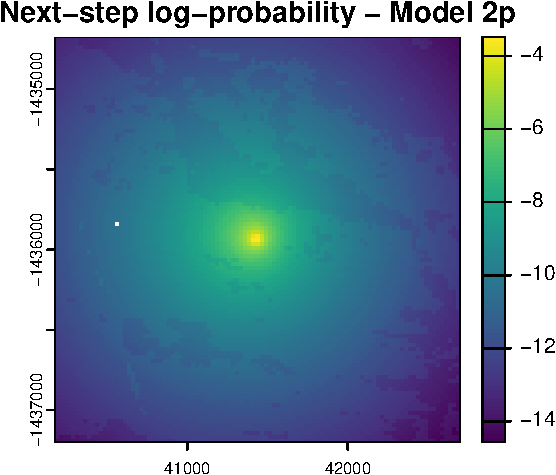
\includegraphics[keepaspectratio]{ssf_validation_files/figure-pdf/unnamed-chunk-8-40.pdf}}

\pandocbounded{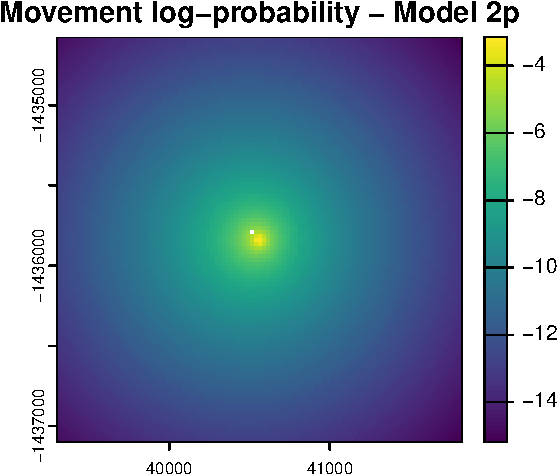
\includegraphics[keepaspectratio]{ssf_validation_files/figure-pdf/unnamed-chunk-8-41.pdf}}

\pandocbounded{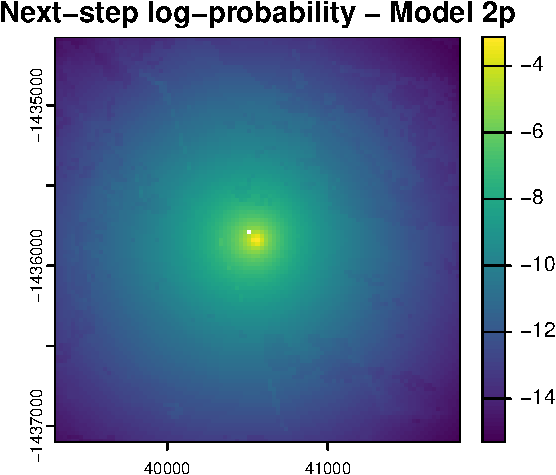
\includegraphics[keepaspectratio]{ssf_validation_files/figure-pdf/unnamed-chunk-8-42.pdf}}

\begin{verbatim}
22.34 sec elapsed
\end{verbatim}

\begin{Shaded}
\begin{Highlighting}[]
\FunctionTok{toc}\NormalTok{()}
\end{Highlighting}
\end{Shaded}

\begin{verbatim}
59.37 sec elapsed
\end{verbatim}

\begin{Shaded}
\begin{Highlighting}[]
\NormalTok{test\_data\_correction }\OtherTok{\textless{}{-}}\NormalTok{ test\_data }\SpecialCharTok{\%\textgreater{}\%} \FunctionTok{drop\_na}\NormalTok{(prob\_habitat\_ssf\_0p) }\SpecialCharTok{\%\textgreater{}\%} 
  \FunctionTok{select}\NormalTok{(t\_, }
\NormalTok{         prob\_habitat\_ssf\_0p, prob\_habitat\_ssf\_2p,}
\NormalTok{         prob\_movement\_ssf\_0p, prob\_movement\_ssf\_2p,}
\NormalTok{         prob\_next\_step\_ssf\_0p, prob\_next\_step\_ssf\_2p}
\NormalTok{         ) }\SpecialCharTok{\%\textgreater{}\%}
  \FunctionTok{mutate}\NormalTok{(}\AttributeTok{t\_ =}\NormalTok{ lubridate}\SpecialCharTok{::}\FunctionTok{as\_datetime}\NormalTok{(t\_)) }\SpecialCharTok{\%\textgreater{}\%} 
  \FunctionTok{pivot\_longer}\NormalTok{(}\AttributeTok{cols =} \SpecialCharTok{!}\FunctionTok{c}\NormalTok{(t\_),}
             \AttributeTok{names\_to =} \StringTok{"model"}\NormalTok{, }\AttributeTok{values\_to =} \StringTok{"prob"}\NormalTok{)}

\FunctionTok{ggplot}\NormalTok{() }\SpecialCharTok{+}
  \FunctionTok{geom\_hline}\NormalTok{(}\AttributeTok{yintercept =} \FloatTok{0.000098}\NormalTok{, }\AttributeTok{linetype =} \StringTok{"dashed"}\NormalTok{) }\SpecialCharTok{+}
  \FunctionTok{geom\_line}\NormalTok{(}\AttributeTok{data=}\NormalTok{test\_data\_correction }\SpecialCharTok{\%\textgreater{}\%} \FunctionTok{filter}\NormalTok{(), }
            \FunctionTok{aes}\NormalTok{(}\AttributeTok{x =}\NormalTok{ t\_, }\AttributeTok{y =}\NormalTok{ prob, }\AttributeTok{colour =}\NormalTok{ model)) }\SpecialCharTok{+}
  \FunctionTok{theme\_bw}\NormalTok{()}
\end{Highlighting}
\end{Shaded}

\begin{verbatim}
Warning: Removed 4 rows containing missing values or values outside the scale range
(`geom_line()`).
\end{verbatim}

\pandocbounded{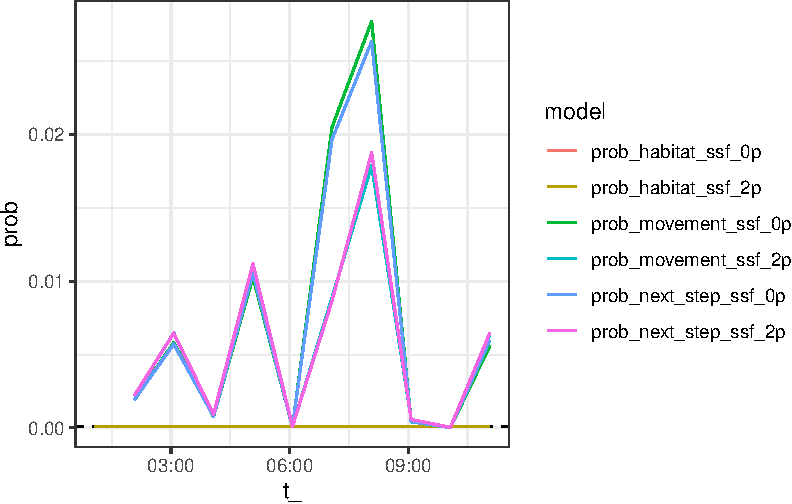
\includegraphics[keepaspectratio]{ssf_validation_files/figure-pdf/unnamed-chunk-9-1.pdf}}

\begin{Shaded}
\begin{Highlighting}[]
\NormalTok{test\_data\_correction }\OtherTok{\textless{}{-}}\NormalTok{ test\_data }\SpecialCharTok{\%\textgreater{}\%} \FunctionTok{drop\_na}\NormalTok{(prob\_habitat\_ssf\_0p) }\SpecialCharTok{\%\textgreater{}\%} 
  \FunctionTok{select}\NormalTok{(t\_, }
\NormalTok{         prob\_habitat\_ssf\_0p, prob\_habitat\_ssf\_2p}
         \CommentTok{\# prob\_movement\_ssf\_0p, prob\_movement\_ssf\_2p,}
         \CommentTok{\# prob\_next\_step\_ssf\_0p, prob\_next\_step\_ssf\_2p}
\NormalTok{         ) }\SpecialCharTok{\%\textgreater{}\%}
  \FunctionTok{mutate}\NormalTok{(}\AttributeTok{t\_ =}\NormalTok{ lubridate}\SpecialCharTok{::}\FunctionTok{as\_datetime}\NormalTok{(t\_)) }\SpecialCharTok{\%\textgreater{}\%} 
  \FunctionTok{pivot\_longer}\NormalTok{(}\AttributeTok{cols =} \SpecialCharTok{!}\FunctionTok{c}\NormalTok{(t\_),}
             \AttributeTok{names\_to =} \StringTok{"model"}\NormalTok{, }\AttributeTok{values\_to =} \StringTok{"prob"}\NormalTok{)}

\FunctionTok{ggplot}\NormalTok{() }\SpecialCharTok{+}
  \FunctionTok{geom\_hline}\NormalTok{(}\AttributeTok{yintercept =} \FloatTok{0.000098}\NormalTok{, }\AttributeTok{linetype =} \StringTok{"dashed"}\NormalTok{) }\SpecialCharTok{+}
  \FunctionTok{geom\_line}\NormalTok{(}\AttributeTok{data=}\NormalTok{test\_data\_correction }\SpecialCharTok{\%\textgreater{}\%} \FunctionTok{filter}\NormalTok{(), }
            \FunctionTok{aes}\NormalTok{(}\AttributeTok{x =}\NormalTok{ t\_, }\AttributeTok{y =}\NormalTok{ prob, }\AttributeTok{colour =}\NormalTok{ model)) }\SpecialCharTok{+}
  \FunctionTok{theme\_bw}\NormalTok{()}
\end{Highlighting}
\end{Shaded}

\pandocbounded{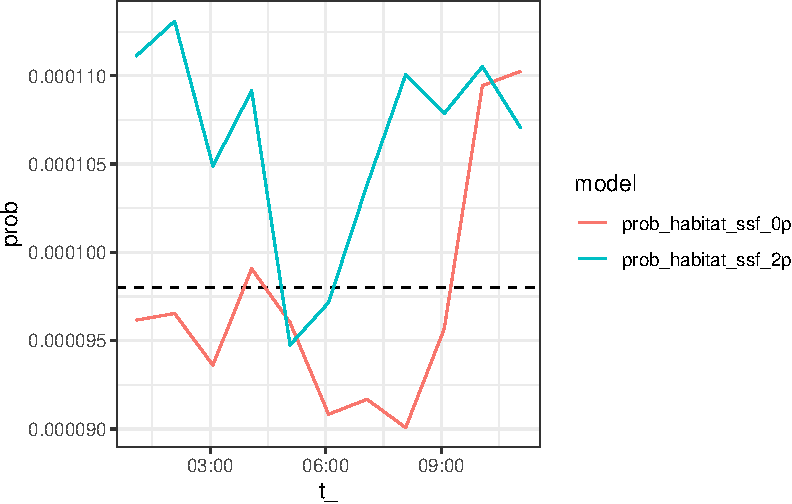
\includegraphics[keepaspectratio]{ssf_validation_files/figure-pdf/unnamed-chunk-9-2.pdf}}




\end{document}
